\documentclass[11pt, aspectratio=169]{beamer}
%
% Choose how your presentation looks.
\usepackage{pgfpages}
\setbeameroption{hide notes}

\usepackage{helvet}
\usepackage{threeparttable}
\usepackage[default]{lato}
\usepackage{array}
\usepackage{tikz}
\usepackage{verbatim}
\usetikzlibrary{positioning}
\usetikzlibrary{calc}
\usetikzlibrary{arrows}
\usetikzlibrary{decorations.markings}
\usetikzlibrary{shapes.misc}
\usetikzlibrary{matrix,shapes,arrows,fit,tikzmark}
\usepackage{amssymb}
\usepackage{amsfonts}
\usepackage{amsmath}
\usepackage{mathpazo}
\usepackage{hyperref}
\usepackage{lipsum}
\usepackage{multimedia}
\usepackage{graphicx}
\usepackage{multirow}
\usepackage{graphicx}
\usepackage{dcolumn}
\usepackage{bbm}
\usepackage{changepage}
\usepackage{appendixnumberbeamer}

\definecolor{blue}{RGB}{0,114,178}
\definecolor{red}{RGB}{213,94,0}
\definecolor{yellow}{RGB}{240,228,66}
\definecolor{green}{RGB}{0,158,115}
\definecolor{gray}{RGB}{240,240,240}

\hypersetup{
  colorlinks={true},
  citecolor=green,
  linkbordercolor = {white},
  linkcolor = {blue}
}

\definecolor{MyBackground}{RGB}{255,253,218}

\newenvironment{transitionframe}{
  \setbeamercolor{background canvas}{bg=gray}
  \begin{frame}}{
    \end{frame}
}

\setbeamercolor{frametitle}{fg=blue}
\setbeamercolor{title}{fg=black}
\setbeamertemplate{footline}[frame number]
\setbeamertemplate{navigation symbols}{} 
\setbeamertemplate{itemize items}{-}
\setbeamercolor{itemize item}{fg=blue}
\setbeamercolor{itemize subitem}{fg=blue}
\setbeamercolor{enumerate item}{fg=blue}
\setbeamercolor{enumerate subitem}{fg=blue}
\setbeamercolor{button}{bg=MyBackground,fg=blue,}
\setbeamercolor{section in toc}{fg=blue}
\setbeamercolor{subsection in toc}{fg=red}
\setbeamersize{text margin left=1em,text margin right=1em} 

\newenvironment{wideitemize}{\itemize\addtolength{\itemsep}{10pt}}{\enditemize}

\mode<presentation>

% \AtBeginSection[]
% {
%   \begin{frame}
%        \frametitle{Contents}
%        \tableofcontents[currentsection]
%   \end{frame}
% }

% \AtBeginSubsection[]
% {
%   \begin{frame}
%        \frametitle{Contents}
%        \tableofcontents[currentsubsection]
%   \end{frame}
% }

\graphicspath{{Graphs/}}

\usepackage[english]{babel}
\usepackage[utf8]{inputenc}
\usepackage[T1]{fontenc}
\usepackage{makecell}
\usepackage{booktabs}
\usepackage[natbibapa]{apacite}

\def\bibfont{\scriptsize}

\title[Your Short Title]{\textcolor{blue}{Pensions and health}}
\author{Arlen Guarin \inst{1} \and Christian Posso \inst{2} \and Pablo Uribe \inst{1}}
\institute{\inst{1} World Bank \and \inst{2} Banco de la República}
\date{May 30, 2024} %\today

\begin{document}

\tikzset{   
        every picture/.style={remember picture,baseline},
        every node/.style={anchor=base,align=center,outer sep=1.5pt},
        every path/.style={thick},
        }
\newcommand\marktopleft[1]{%
    \tikz[overlay,remember picture] 
        \node (marker-#1-a) at (-.3em,.3em) {};%
}
\newcommand\markbottomright[2]{%
    \tikz[overlay,remember picture] 
        \node (marker-#1-b) at (0em,0em) {};%
}
\tikzstyle{every picture}+=[remember picture] 
\tikzstyle{mybox} =[draw=black, very thick, rectangle, inner sep=10pt, inner ysep=20pt]
\tikzstyle{fancytitle} =[draw=black,fill=red, text=white]

\begin{frame}
  \maketitle
\end{frame}

\begin{frame}
    \frametitle{Contents}
    \tableofcontents
\end{frame}

%%%%%%%%%%%%%%%%% Introduction

\section{Introduction}

\begin{transitionframe}
  \begin{center}
    { \huge \textcolor{blue}{Introduction}}
  \end{center}
\end{transitionframe}

\begin{frame}{Introduction}
    \begin{wideitemize}
        \item There is a lot of evidence on the effects of pension reforms on labor market outcomes {\footnotesize \citep{hernaes2016pension,fisher2010pension,sanchez2014delaying,geyer2020labor}}.
        \item Interesting cross-country correlations between retirement and health {\footnotesize \citep{coe2011retirement}}.
        \item Scarce and inconclusive evidence on the effects of increasing retirement age on the health and well-being of older workers {\footnotesize \citep{pilipiec2021effect}}.
        \begin{itemize}
            \item \textbf{Highlight:} Admin data from Sweden $\longrightarrow$ No effects on mortality or healthcare utilization {\footnotesize \citep{hagen2018effects}}.
        \end{itemize}
        \item No evidence of negative effects of post-retirement age working on mental health. Some evidence of positive effects {\footnotesize \citep{maimaris2010impact}}.
        \begin{itemize}
            \item \textbf{Potential mechanisms:} Maintenance of productive roles, continued income, and continued social support.
        \end{itemize}
    \end{wideitemize}

\end{frame}


%%%%%%%%%%%%%%%%% Context

\section{Context}

\begin{transitionframe}
  \begin{center}
    { \huge \textcolor{blue}{Context}}
  \end{center}
\end{transitionframe}

\begin{frame}{Context}
    \textbf{Law 100 of 1993}
    \vspace{0.2cm}
    \begin{itemize}
        \item \textbf{ARTICLE 33.} \underline{Pension Requirements}:
        \begin{wideitemize}
            \item Must be fifty-five (55) years old if female, or sixty (60) years old if male.
            \item Must have contributed for a minimum of 1,000 weeks at any time.
            \item \textbf{PARAGRAPH 4.} Starting from January 1, 2014, the ages for accessing the old-age pension will be adjusted to fifty-seven (57) years if female and sixty-two (62) years if male.
        \end{wideitemize}
    \end{itemize}

\end{frame}

\begin{frame}{Context}
    \begin{itemize}
        \item \textbf{ARTICLE 36.} \underline{Transition Regime.} The age for accessing the old-age pension will remain fifty-five (55) years for women and sixty (60) years for men, until the year 2014, at which point the age will increase by 2 years, meaning it will be 57 years for women and 62 for men.
        \begin{itemize}
            \item The provisions of this article will not apply to individuals who, at the time the regime comes into effect, are thirty-five (35) or more years old if female or forty (40) or more years old if male, \textbf{unless these individuals voluntarily choose to join the individual savings regime with solidarity}, in which case they will be subject to all the conditions set forth for that regime.
            \item One of the requirements is to be 35-40 years old but it is also possible to enter the regime if, at the time it comes into effect, one has 15 or more years of contributions (750 weeks).
        \end{itemize}
    \end{itemize}
\end{frame}

\begin{frame}{Context}
\textbf{Legislative Act 01 of 2005}

    \begin{itemize}
        \item \textbf{Transitional Paragraph 4.} The transition regime established in Law 100 of 1993 and other regulations that develop this regime, cannot be extended beyond July 31, 2010; except for workers who are in this regime and have also contributed at least 750 weeks or the equivalent in service time by the time this Legislative Act comes into effect, in which case the regime will be maintained until the year 2014.
        \item The privileged pension regimes are eliminated, except those applicable to members of the Public Force and the President of the Republic.
        \item Teachers will continue to retire according to the provisions of Law 812 of 2003 or the National Development Plan. This means that teachers appointed before June 27, 2003 will continue to retire at the age of 55 for men and 50 for women, with 75 percent of the average salary of the last year.
    \end{itemize}
\end{frame}

\begin{frame}{Context}

    \begin{itemize}
        \item Regarding the transition regime for obtaining the pension, it was approved that the elimination of this regime \textbf{is moved forward from the year 2014 to July 31, 2010}, but it is maintained until 2014 for individuals who have contributed a minimum of 15 years or 750 weeks.
        \item Maintaining this transition regime until July 31, 2010 implies that women who were 35 years old in 1994, men who were 40 years old or had 15 years of contributions, will retire at 55 years old for women and 60 years old for men. $\longrightarrow$ To be eligible for the extension to 2014, one must have at least 750 weeks of contributions by today (July 25, 2005).
    \end{itemize}

    \textit{Note:} The transition regime (RT) must be extended until December 31, 2014: \textit{Consejo de Estado}.

\end{frame}

\begin{frame}{Context}
\textbf{Example cohort 50}

    Suppose they do not meet the 750 weeks of contributions:

    \begin{enumerate}
        \item Man born on July 31, 1950 $\longrightarrow$ In 1994 he is 44 years old (meets the requirement for transition). On July 31, 2010 he turns 60 years old and \textbf{can retire with the RT.}
        \item Man born on August 1, 1950 $\longrightarrow$ In 1994 he is 44 years old (meets the requirement for transition). On July 31, 2010 he is not yet 60 years old and \textbf{cannot retire with the RT unless he had the weeks}. He would retire in 2012 at the age of 62.
    \end{enumerate}

\end{frame}

\begin{frame}{Context}
    \textbf{Example cohort 54}

    \begin{enumerate}
        \item Man born on April 1, 1954 $\longrightarrow$ On April 1, 1994 he turns 40 and enters the RT. On July 31, 2010 he does not meet the age requirement, \textbf{he can only retire at 60 if he has 750 weeks} by July 25, 2005.
        \item Man born between April 2 and December 31, 1954 $\longrightarrow$ On April 1, 1994 he is 39 years old. \textbf{The only way to enter the RT is to have 15 years of service contributions by that date}. He would be eligible for a pension in 2014 at the age of 60.
        \item Man born on January 1, 1955 $\longrightarrow$ On April 1, 1994 he is 39 years old. The only way to enter the RT is to have 15 years of service contributions by that date. However, under Legislative Act 01 of 2005, \textbf{he would not be able to retire at 60 even if he had the weeks}, since on December 31, 2014 he would be 59 years old.
    \end{enumerate}
\end{frame}

\begin{frame}{Timeline}
\begin{center}
\begin{tikzpicture}[font=\scriptsize]

% Define coordinates for cut points on the timeline
\coordinate (A) at (0, 0);
\coordinate (B) at (3, 0);
\coordinate (C) at (6, 0);
\coordinate (D) at (9, 0);
\coordinate (E) at (12, 0);
\coordinate (F) at (13, 0); % Extended point for arrow

% Draw the timeline
\draw[thick] (A) -- (E);
\draw[thick, ->] (E) -- ++(1,0); % Arrow at the end

% Draw cut points and labels
\only<1->{\fill (A) circle (2pt) node[below] {1993};}
\only<2->{\fill (B) circle (2pt) node[above] {April 1 \\ 1994};}
\only<3->{\fill (C) circle (2pt) node[below] {2005 \\ July 25};}
\only<4->{\fill (D) circle (2pt) node[above] {July 31 \\ 2010};}
\only<5->{\fill (E) circle (2pt) node[below] {2014 \\ December 31};}

% Draw lines and bubbles for text
\only<1->{\draw (A) -- ++(0, 1) node[draw=blue, rectangle, fill=white, rounded corners, text width=2cm, align=center] {{\tiny \textbf{Law 100}: Introduces TR}};}
\only<2->{\draw (B) -- ++(0, -1) node[draw=blue, rectangle, fill=white, rounded corners, text width=2cm, align=center] {{\tiny \textbf{Conditions for TR:}\\40 yo men or 35 yo women. If <age, >750 weeks}};}
\only<3->{\draw (C) -- ++(0, 2.5) node[draw=blue, rectangle, fill=white, rounded corners, text width=2cm, align=center] {{\tiny \textbf{Legislative Act 01:}\\TR to extend only until July 31, 2010. Unless >750 weeks. Then, extends to 2014.}};}
\only<4->{\draw (D) -- ++(0, -1) node[draw=blue, rectangle, fill=white, rounded corners, text width=2cm, align=center] {{\tiny If TR and >= 60/55, then retirement.\\If <60/55 and <750 weeks by 2005, retirement age is increased by 2 years.}};}
\only<5->{\draw (E) -- ++(0, 1.5) node[draw=blue, rectangle, fill=white, rounded corners, text width=2cm, align=center] {{\tiny TR ends and age is increased by 2 years.}};}

\end{tikzpicture}
\end{center}

\vfill
{\scriptsize TR: Transition Regime.}

\end{frame}


%%%%%%%%%%%%%%% Data

\section{Data}

\begin{transitionframe}
  \begin{center}
    { \huge \textcolor{blue}{Data}}
  \end{center}
\end{transitionframe}

\begin{frame}{Master data}
    \begin{wideitemize}
        \item Population of formal workers between 2008 and 2022 that meet these criteria: 
        \begin{enumerate}
            \item Men born between 1948-1952 (M50) $\longrightarrow$ Cutoff date: July 31, 1950.
            \item Men born between 1952-1956 (M54) $\longrightarrow$ Cutoff date: April 1, 1954.
            \item Women born between 1953-1957 (F55) $\longrightarrow$ Cutoff date: July 31, 1955.
            \item Women born between 1957-1961 (F59) $\longrightarrow$ Cutoff date: April 1, 1959.
        \end{enumerate}
        \item Due to a mass accumulation of birth dates on January 1, we decide to drop those observations to avoid contamination (``donut hole'').
        \item Running variable is created as the difference in weeks between the DOB and the cutoff date.
        \item We will focus on the M50 and F55 cohorts, since they are the cleanest.
    \end{wideitemize}
\end{frame}

\begin{frame}{Health data - RIPS}
    \begin{wideitemize}
        \item Take all available RIPS years (2009-2022) from its four datasets:
        \begin{itemize}
            \item Consultations.
            \item Procedures.
            \item Emergencies.
            \item Hospitalizations.
        \end{itemize}
        \item Keep only people from our master sample.
        \item Use the diagnosis codes to create all relevant outcomes. 
        \item Keep only one observation per person by reshaping the data (number of records is saved as the intensive margin).
        \item We then balance the dataset at the person-age level.
    \end{wideitemize}
\end{frame}

\begin{frame}{Census microdata (baseline)}
    \begin{wideitemize}
        \item Data retrieved from IPUMS.
        \item 1993 census does not have birth dates, so the running variable can't be created.
        \item 2005 census contains month and year of birth.
        \item This data is the closest we can get to baseline data. It will allow us to perform balance tests.
    \end{wideitemize}
\end{frame}



%%%%%%%%%%%%%%%%%%%%%%% Empirical strategy

\section{Empirical strategy}

\begin{transitionframe}
  \begin{center}
    { \huge \textcolor{blue}{Empirical strategy}}
  \end{center}
\end{transitionframe}

\begin{frame}{Empirical strategy}
If there are specific cutoffs that determine eligibility for X policy $\longrightarrow$ Regression discontinuity design (RDD).

Local polynomial approach:
    \begin{equation*}
    Y_i = \alpha + \beta_1 Above_i + h(Z_i) + \varepsilon \quad \forall \quad \mid Z_i \mid <= H
\end{equation*}

\begin{itemize}
    \item This is equivalent to fitting a linear regression on each side of the cutoff. You are using only the observations within some pre-specified window H $\longrightarrow$ Specification bias since true conditional expectation function is likely not linear.
    \item \textbf{Bias-variance trade-off:} The shorter the window, the lower the bias, but because you have less data, the variance in your estimate increases.
    \item Non-parametric methods choose optimal bandwidths that may differ left and right of the cutoff based on the trade-off \textbf{(this is the most common method)}.
\end{itemize}

\vfill
\end{frame}

\begin{frame}{Identification}
    \begin{itemize}
        \item<1-> \textbf{Main challenges to identification:}
    \begin{itemize}
        \item<1-> The assignment rule is known in advance.
        \item<1-> Agents are interested in adjusting.
        \item<1-> Agents have time to adjust.
        \item<1-> The cutoff is endogenous to factors that independently cause potential outcomes to shift.
        \item<1-> There is nonrandom heaping along the running variable.
    \end{itemize}

    \item<2-> The \textbf{McCrary density test} is used to check whether units are sorting on the running variable (i.e., manipulation).
    \item<2-> \textbf{Balance tests} $\longrightarrow$ Pre-treatment characteristics should be invariant to change in treatment assignment (i.e., no effect where there should not be) $\longrightarrow$ \textbf{Placebo tests}.
    \item<2-> When there is nonrandom heaping, a possible solution is doing a \textbf{``donut hole'' RDD} (i.e., remove observations in the vicinity of the heaping values).
     \end{itemize}
\end{frame}

%%%%%%%%%%%%%%%%% Balance
\subsection{Balance}

\begin{transitionframe}
  \begin{center}
    { \huge \textcolor{blue}{Balance and manipulation tests}}
  \end{center}
\end{transitionframe}

\begin{frame}{Balance}
    \begin{wideitemize}
        \item We use the 2005 census data to look at covariate balance in the year that the Legislative Act was passed (baseline).
        \item Non-parametric RD regressions including cohort FE on several health- and work-related outcomes.
    \end{wideitemize}
\end{frame}

\begin{frame}[label=balance]{Balance}
    \centering
    \resizebox{0.65\textwidth}{!}{
      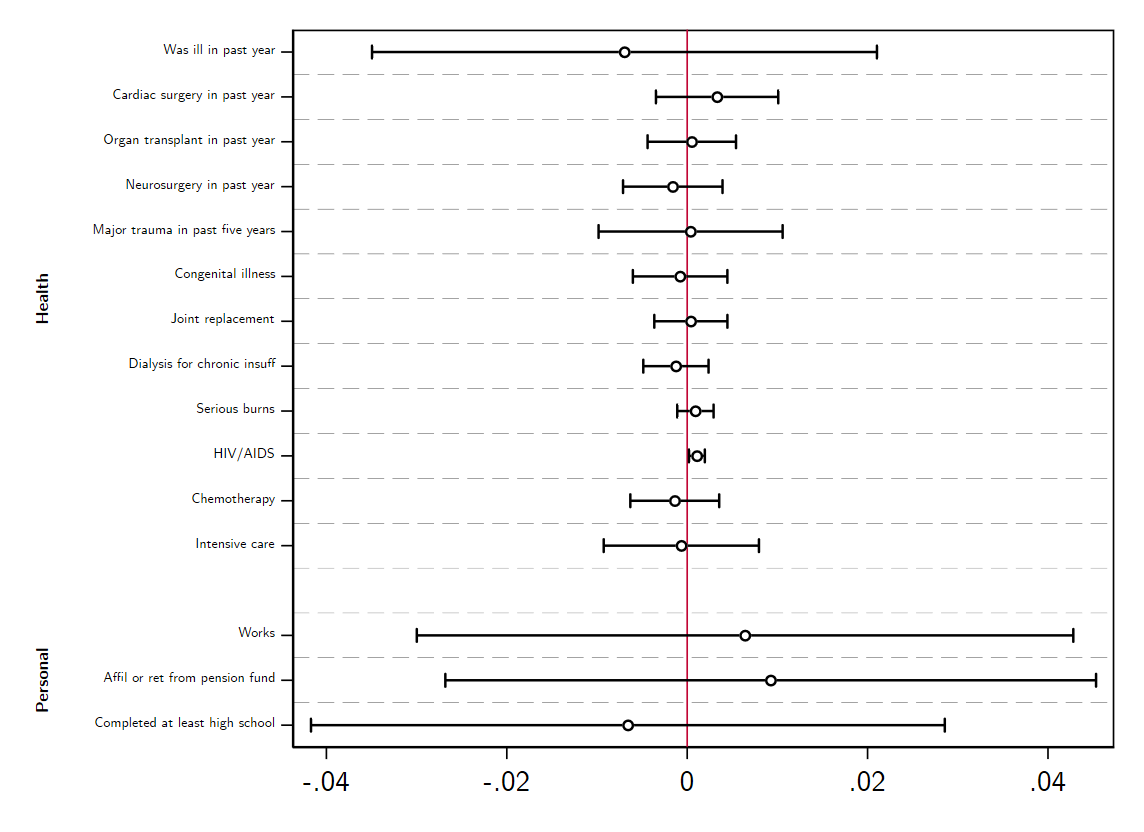
\includegraphics{Graphs/balance_RD_final.png}
    }
    
    \vfill
    \centering
    \hyperlink{m50_balance}{\beamergotobutton{See for M50}}
    \hyperlink{f55_balance}{\beamergotobutton{See for F55}}
\end{frame}


%%%%%%%%%%%%%%% Manipulation
\subsection{Manipulation tests}

\begin{frame}{Manipulation tests}
    \centering
    \resizebox{0.65\textwidth}{!}{
      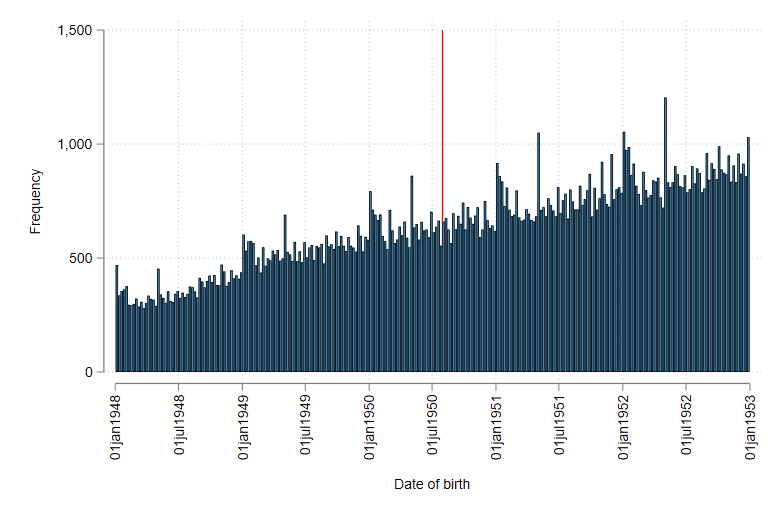
\includegraphics{Graphs/hist_M50.png}
    }
\end{frame}

\begin{frame}{Manipulation tests}
    \centering
    \resizebox{0.65\textwidth}{!}{
      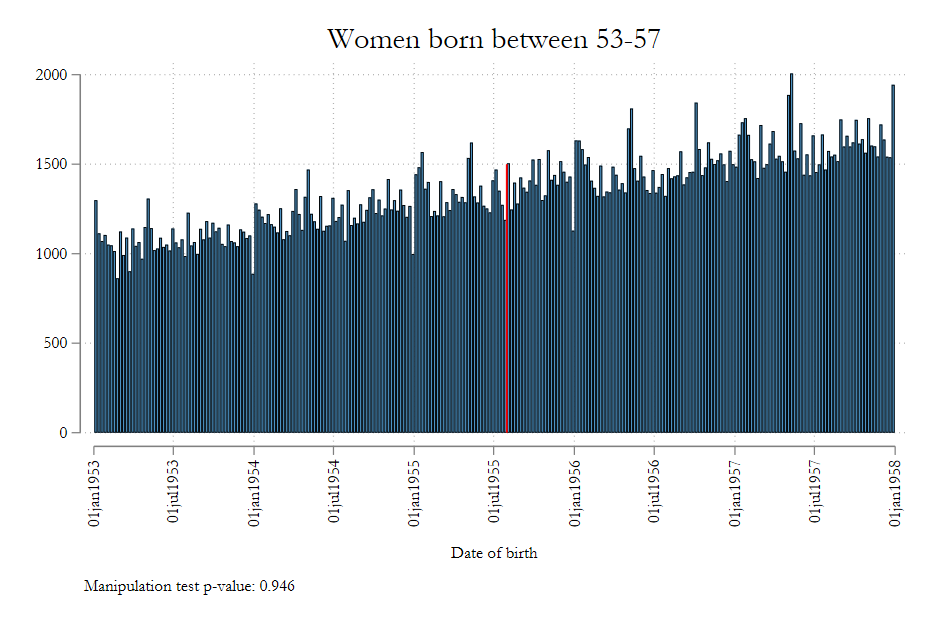
\includegraphics{Graphs/hist_F55.png}
    }
\end{frame}

%%%%%%%%%%%%%%% Results
\section{Health results}

\begin{transitionframe}
  \begin{center}
    { \huge \textcolor{blue}{Health results}}
  \end{center}
\end{transitionframe}

%Consul
\begin{frame}[label=f55_consul]{Health results}
    \centering
    \resizebox{0.8\textwidth}{!}{
      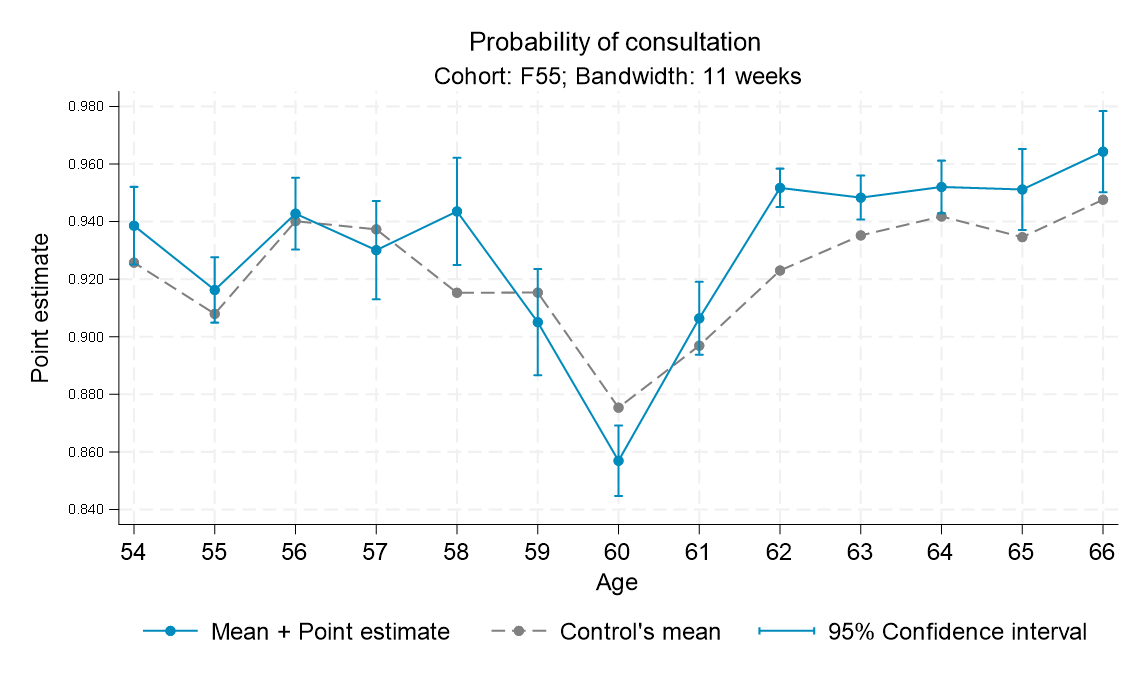
\includegraphics{Graphs/age/consul_F55_11_age.png}
    }
    
    \vfill
    \centering
    \hyperlink{f55_consul_cum}{\beamergotobutton{See cumulative}}
    \hyperlink{f55_nroconsul}{\beamergotobutton{See intensive margin}}
\end{frame}

\begin{frame}[label=m50_consul]{Health results}
    \centering
    \resizebox{0.8\textwidth}{!}{
      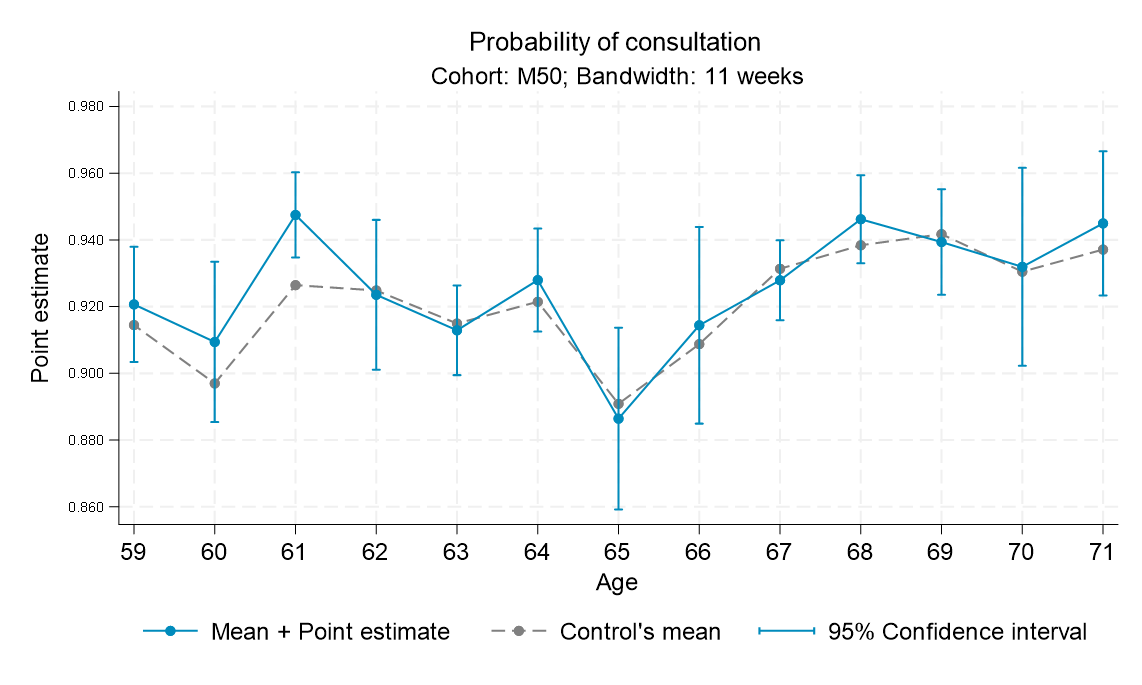
\includegraphics{Graphs/age/consul_M50_11_age.png}
    }
    
    \vfill
    \centering
    \hyperlink{m50_consul_cum}{\beamergotobutton{See cumulative}}
    \hyperlink{m50_nroconsul}{\beamergotobutton{See intensive margin}}
\end{frame}




%Hosp
\begin{frame}[label=f55_hosp]{Health results}
    \centering
    \resizebox{0.8\textwidth}{!}{
      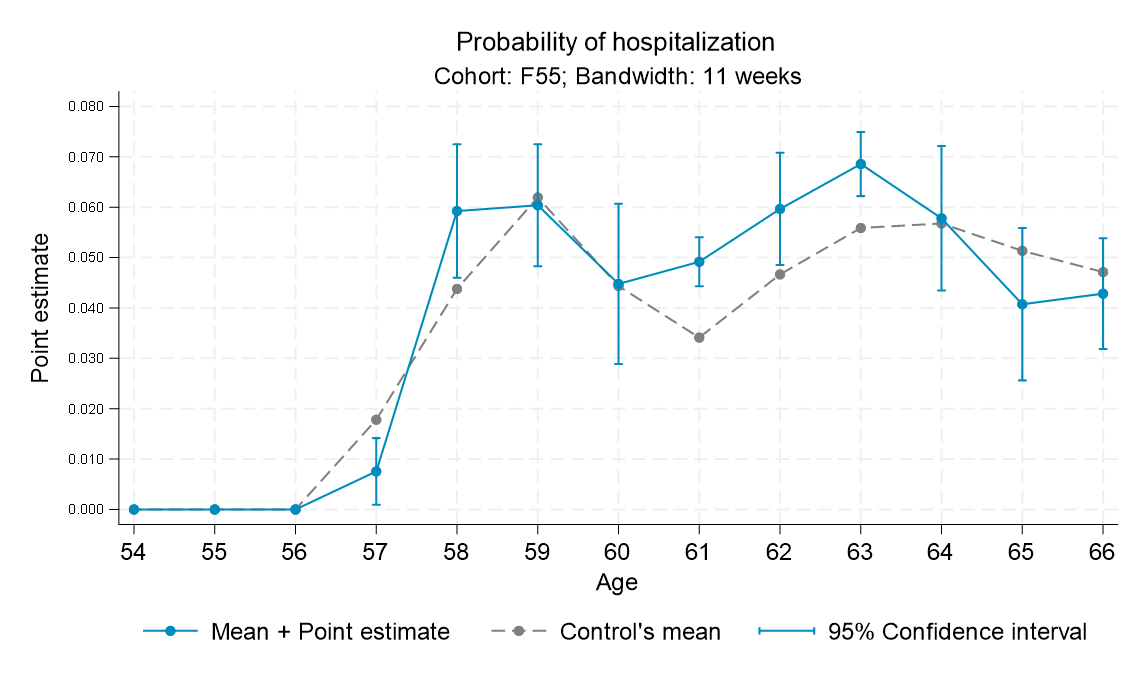
\includegraphics{Graphs/age/hosp_F55_11_age.png}
    }
    
    \vfill
    \centering
    \hyperlink{f55_hosp_cum}{\beamergotobutton{See cumulative}}
    \hyperlink{f55_nrohosp}{\beamergotobutton{See intensive margin}}
\end{frame}

\begin{frame}[label=m50_hosp]{Health results}
    \centering
    \resizebox{0.8\textwidth}{!}{
      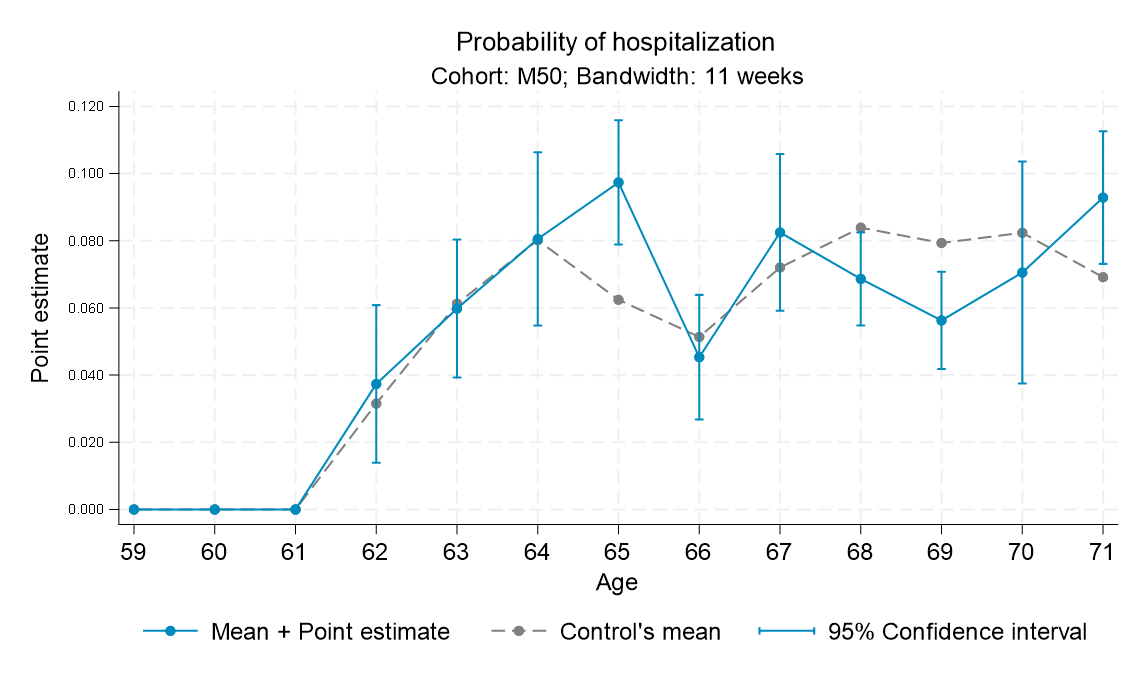
\includegraphics{Graphs/age/hosp_M50_11_age.png}
    }
    
    \vfill
    \centering
    \hyperlink{m50_hosp_cum}{\beamergotobutton{See cumulative}}
    \hyperlink{m50_nrohosp}{\beamergotobutton{See intensive margin}}
\end{frame}





%Cardio
\begin{frame}[label=f55_cardio]{Health results}
    \centering
    \resizebox{0.8\textwidth}{!}{
      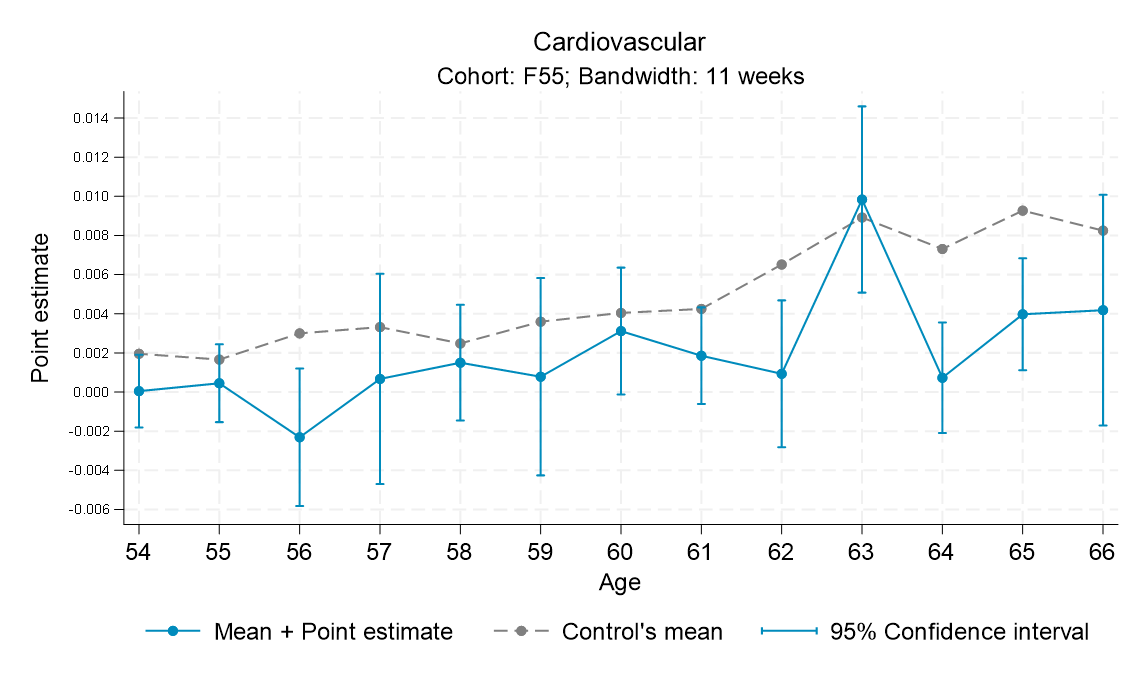
\includegraphics{Graphs/age/cardiovascular_F55_11_age.png}
    }
    
    \vfill
    \centering
    \hyperlink{f55_cardio_cum}{\beamergotobutton{See cumulative}}
\end{frame}

\begin{frame}[label=m50_cardio]{Health results}
    \centering
    \resizebox{0.8\textwidth}{!}{
      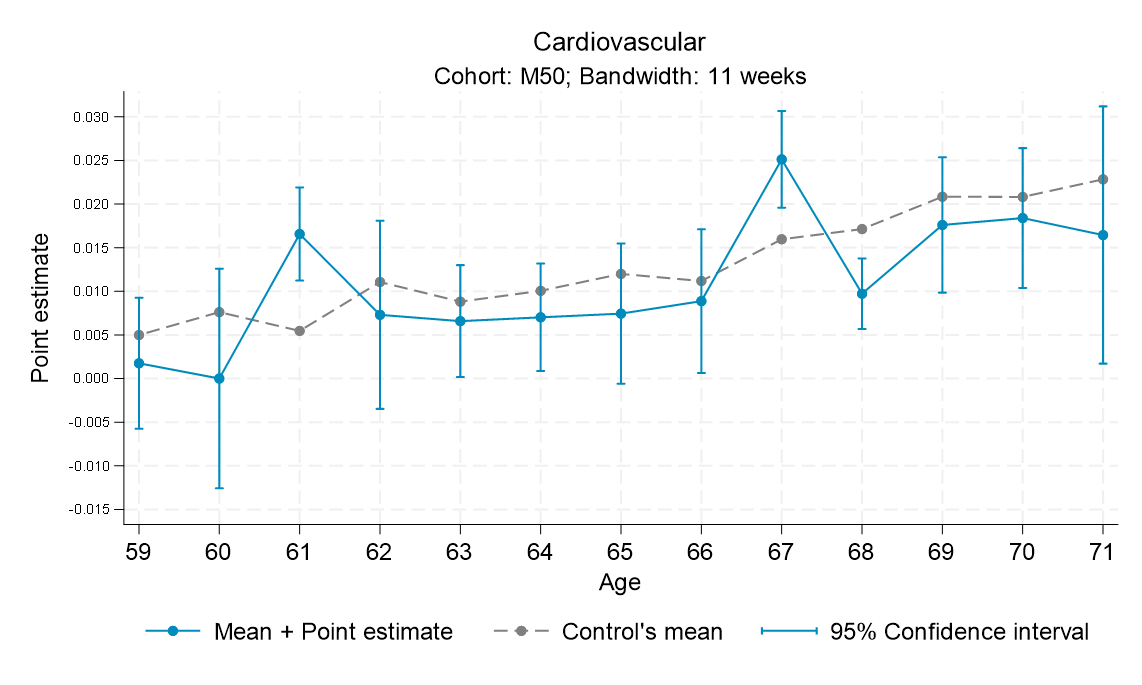
\includegraphics{Graphs/age/cardiovascular_M50_11_age.png}
    }
    
    \vfill
    \centering
    \hyperlink{m50_cardio_cum}{\beamergotobutton{See cumulative}}
\end{frame}



%Infarct
\begin{frame}[label=f55_infarct]{Health results}
    \centering
    \resizebox{0.8\textwidth}{!}{
      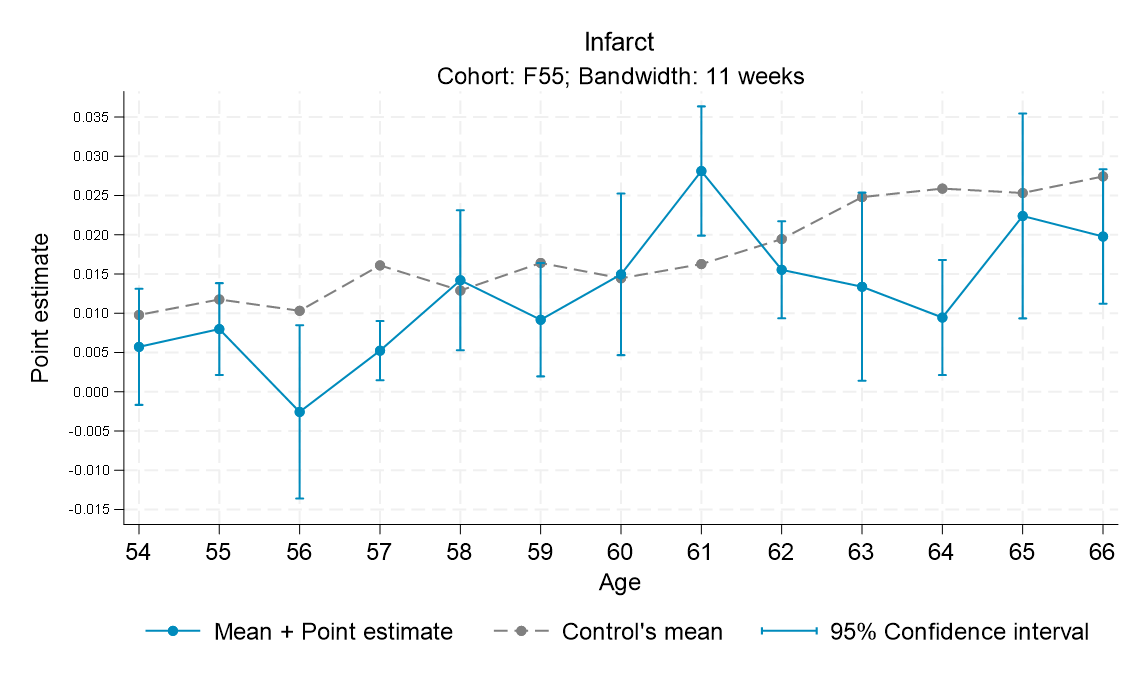
\includegraphics{Graphs/age/infarct_F55_11_age.png}
    }
    
    \vfill
    \centering
    \hyperlink{f55_infarct_cum}{\beamergotobutton{See cumulative}}
\end{frame}

\begin{frame}[label=m50_infarct]{Health results}
    \centering
    \resizebox{0.8\textwidth}{!}{
      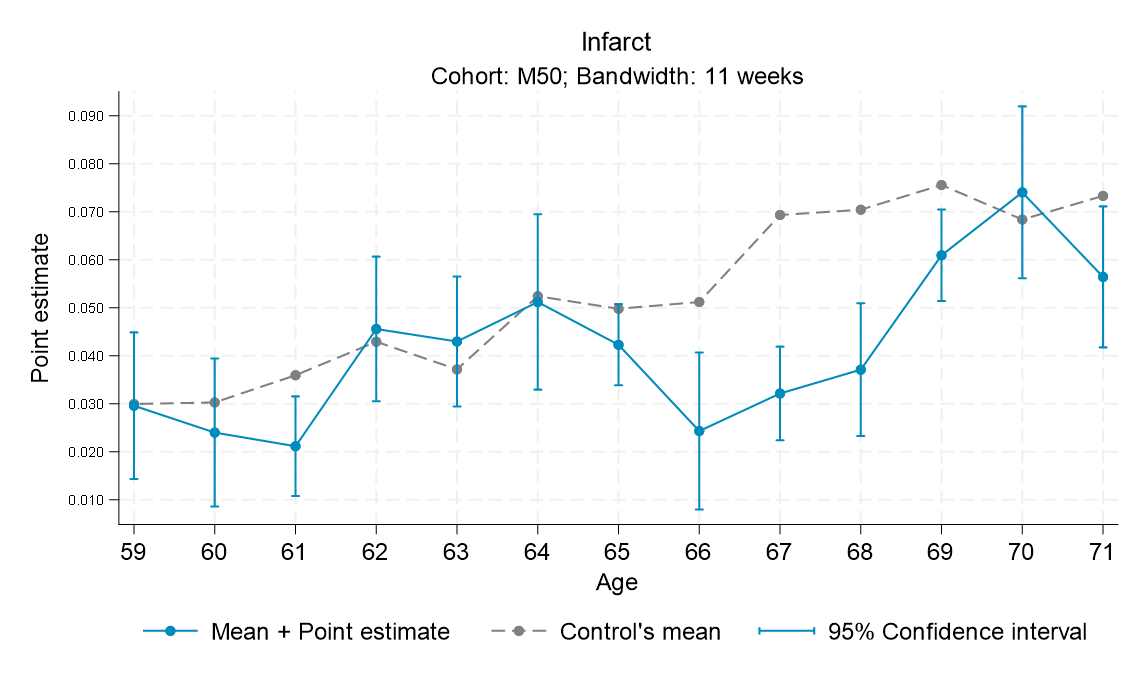
\includegraphics{Graphs/age/infarct_M50_11_age.png}
    }
    
    \vfill
    \centering
    \hyperlink{m50_infarct_cum}{\beamergotobutton{See cumulative}}
\end{frame}


%Stress
\begin{frame}[label=f55_stress]{Health results}
    \centering
    \resizebox{0.8\textwidth}{!}{
      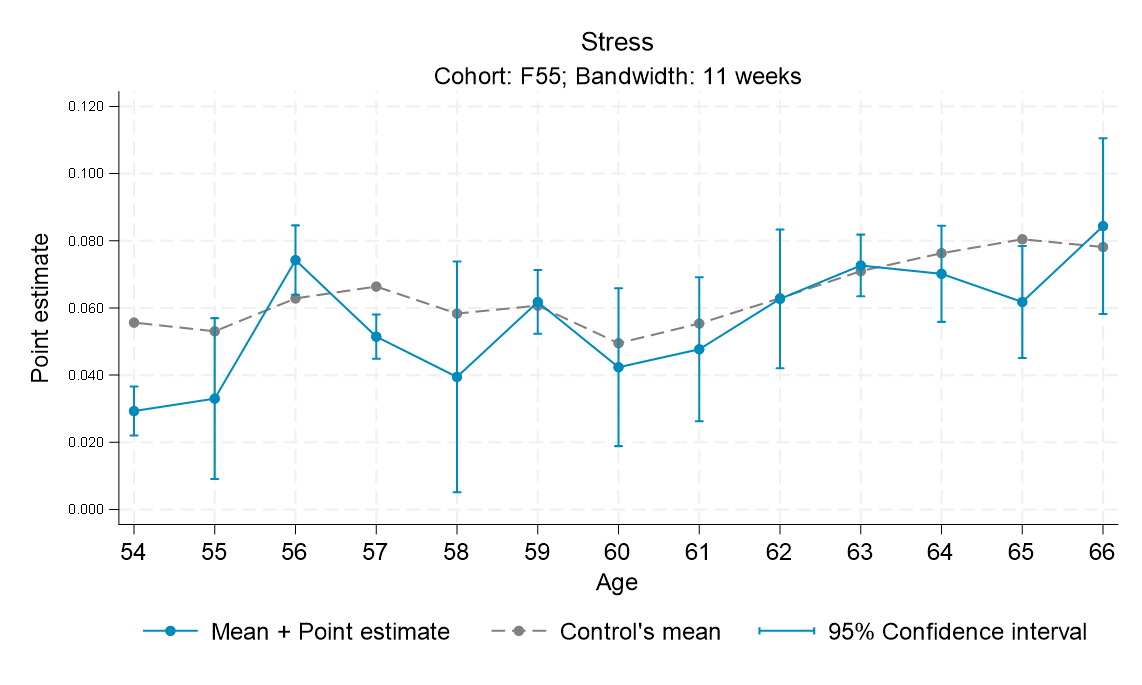
\includegraphics{Graphs/age/estres_F55_11_age.png}
    }
    
    \vfill
    \centering
    \hyperlink{f55_stress_cum}{\beamergotobutton{See cumulative}}
\end{frame}

\begin{frame}[label=m50_stress]{Health results}
    \centering
    \resizebox{0.8\textwidth}{!}{
      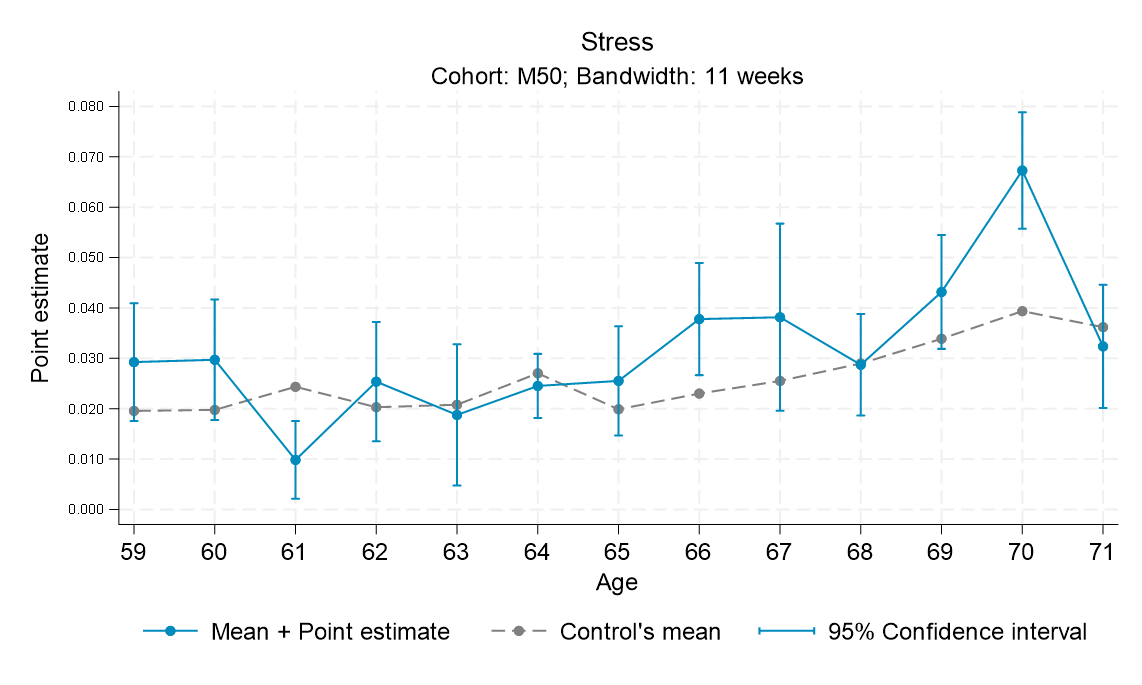
\includegraphics{Graphs/age/estres_M50_11_age.png}
    }
    
    \vfill
    \centering
    \hyperlink{m50_stress_cum}{\beamergotobutton{See cumulative}}
\end{frame}



%Mental diagnosis
\begin{frame}[label=f55_mental]{Health results}
    \centering
    \resizebox{0.8\textwidth}{!}{
      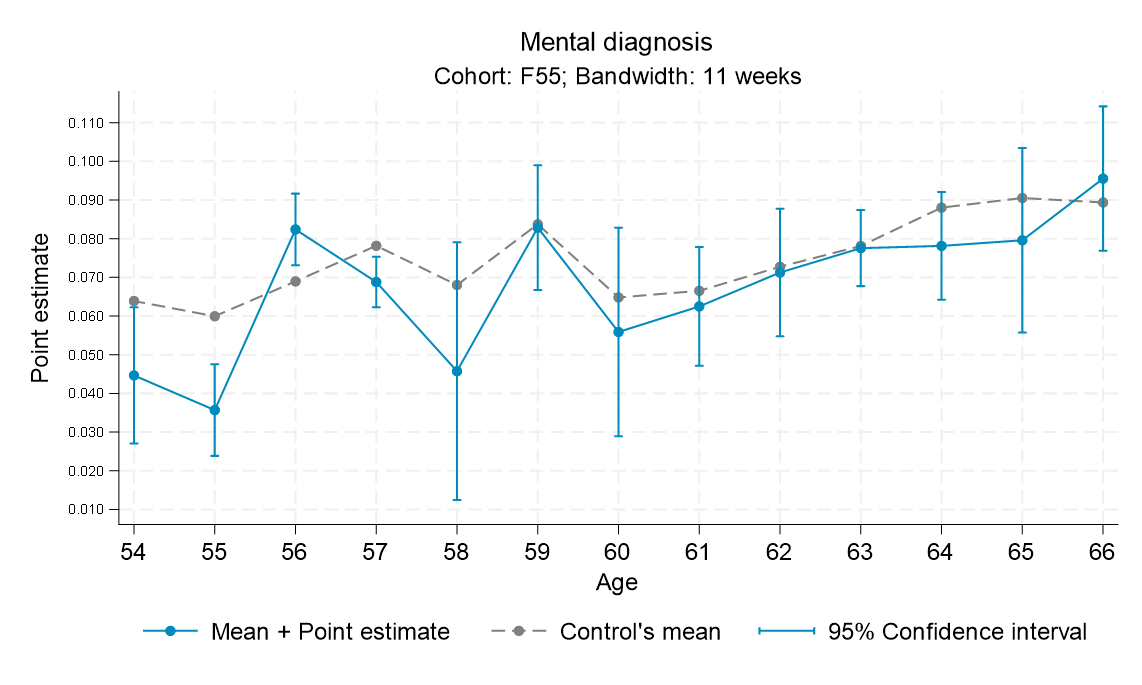
\includegraphics{Graphs/age/diag_mental_F55_11_age.png}
    }
    
    \vfill
    \centering
    \hyperlink{f55_mental_cum}{\beamergotobutton{See cumulative}}
\end{frame}

\begin{frame}[label=m50_mental]{Health results}
    \centering
    \resizebox{0.8\textwidth}{!}{
      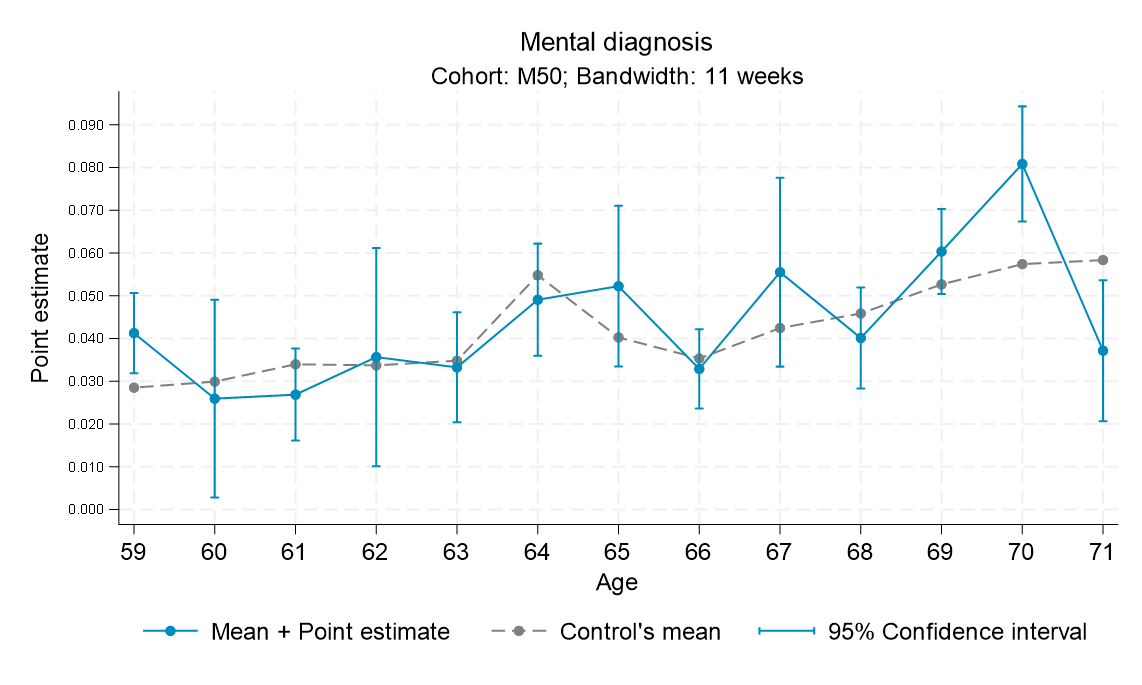
\includegraphics{Graphs/age/diag_mental_M50_11_age.png}
    }
    
    \vfill
    \centering
    \hyperlink{m50_mental_cum}{\beamergotobutton{See cumulative}}
\end{frame}



%MWI
\begin{frame}[label=f55_mwi]{Health results}
    \centering
    \resizebox{0.8\textwidth}{!}{
      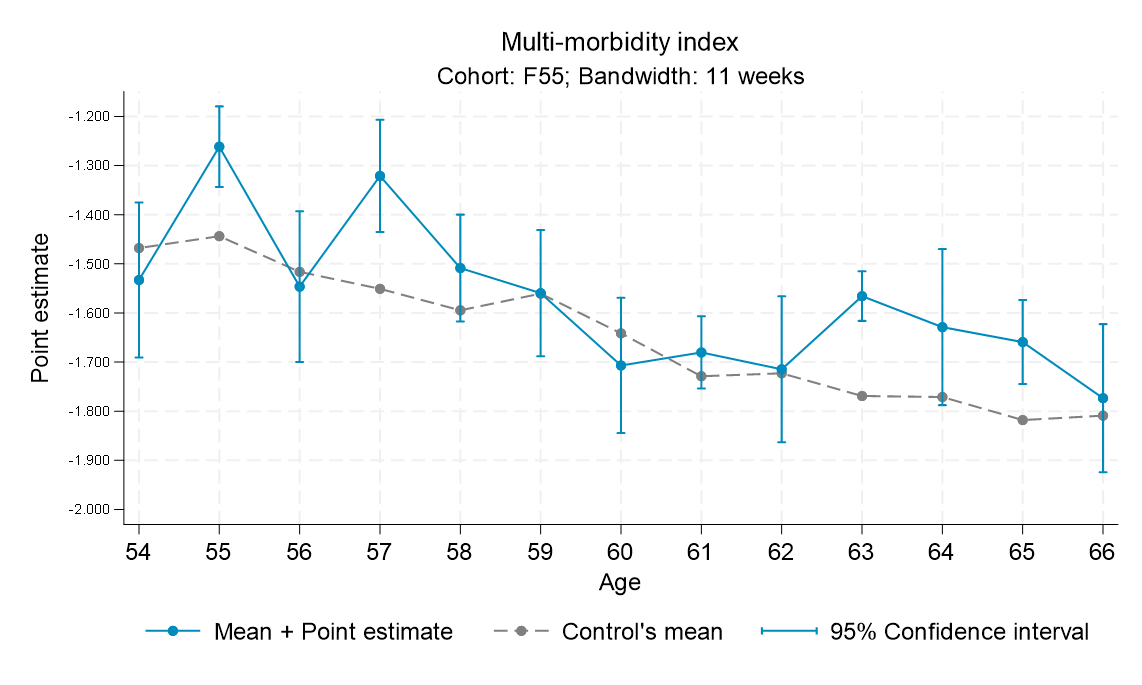
\includegraphics{Graphs/age/pre_MWI_F55_11_age.png}
    }
    
    \vfill
    \centering
    \hyperlink{f55_mwi_cum}{\beamergotobutton{See cumulative}}
\end{frame}

\begin{frame}[label=m50_mwi]{Health results}
    \centering
    \resizebox{0.8\textwidth}{!}{
      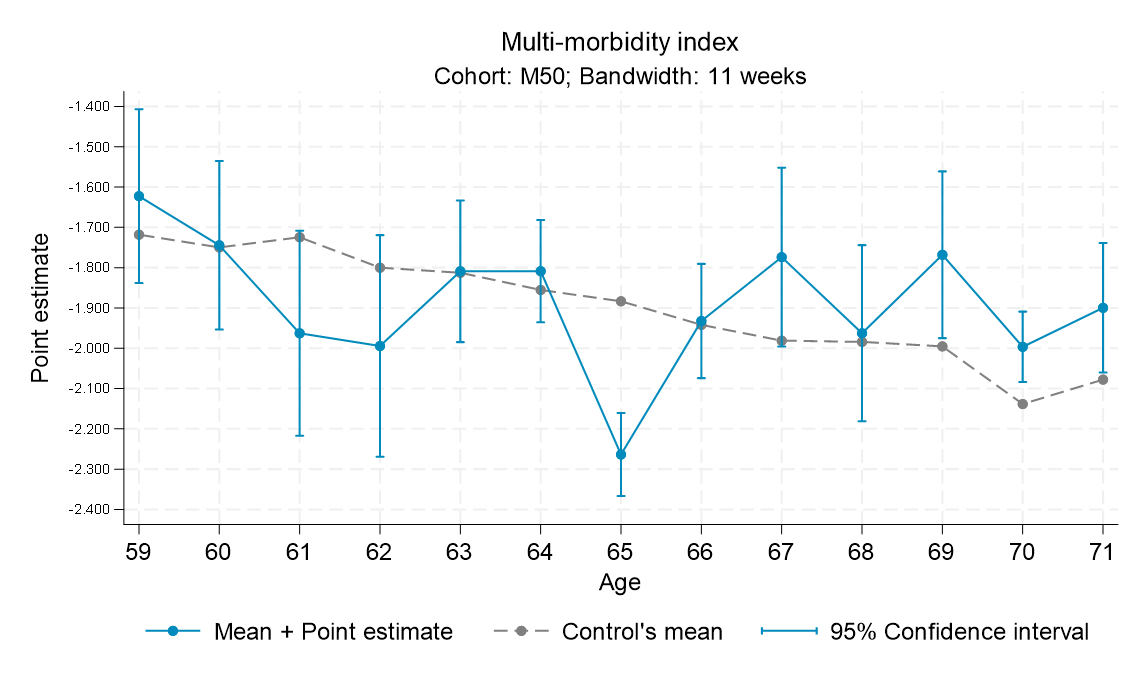
\includegraphics{Graphs/age/pre_MWI_M50_11_age.png}
    }
    
    \vfill
    \centering
    \hyperlink{m50_mwi_cum}{\beamergotobutton{See cumulative}}
\end{frame}



%%%%%%%%%%%%%%% Next steps

\section{Next steps}

\begin{transitionframe}
  \begin{center}
    { \huge \textcolor{blue}{Next steps}}
  \end{center}
\end{transitionframe}

\begin{frame}{Next steps}
    \begin{wideitemize}
        \item Use data from Vital Statistics to estimate the RDD on mortality.
        \item Estimate effects on labor market outcomes like retirement.
        \item Calculate regressions with optimal BW.
        \item Explore potential mechanisms.
        \item Special regimes (?).
        
    \end{wideitemize}
\end{frame}

\section*{References}
\begin{frame}[allowframebreaks]{References}
\bibliographystyle{apacite}
\tiny\bibliography{references}
\end{frame}

\appendix

\begin{frame}[label=m50_balance]{Balance (M50 cohort)}
    \centering
    \resizebox{0.65\textwidth}{!}{
      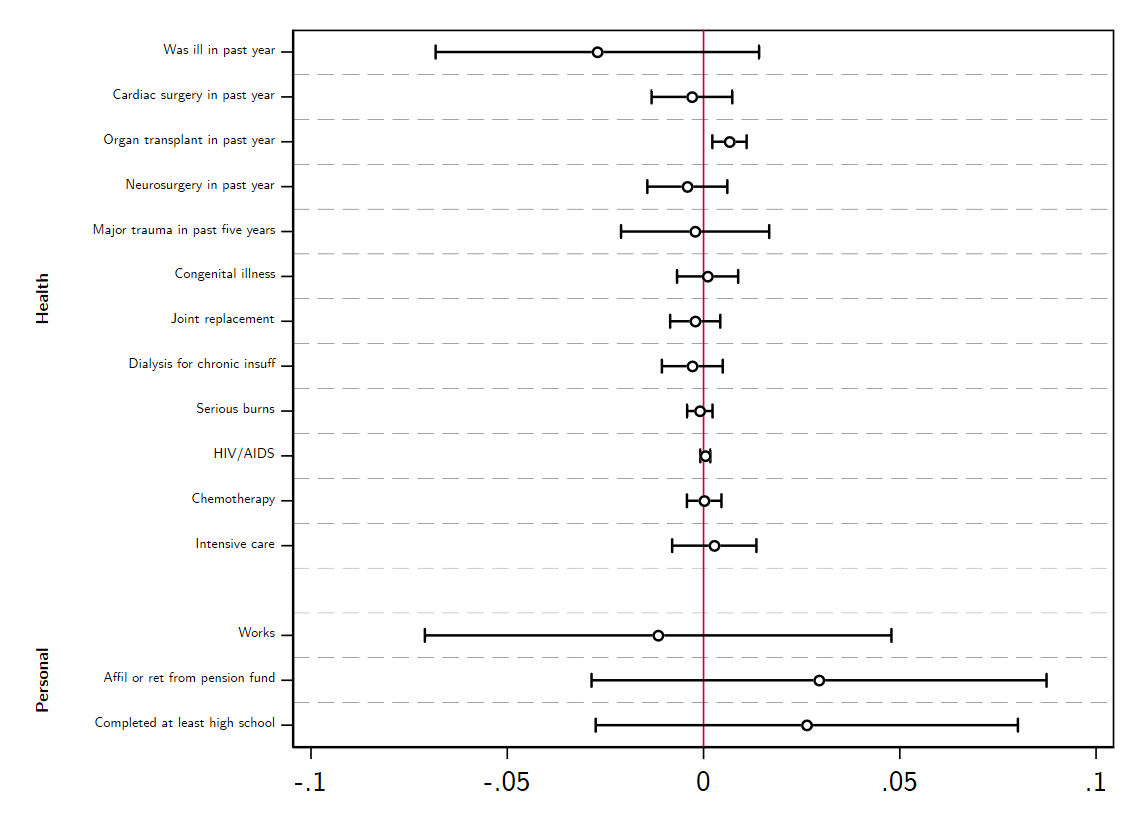
\includegraphics{Graphs/balanceRD_final_M50.png}
    }
    \vfill
    \centering
    \hyperlink{balance}{\beamergotobutton{Back}}
\end{frame}

\begin{frame}[label=f55_balance]{Balance (F55 cohort)}
    \centering
    \resizebox{0.65\textwidth}{!}{
      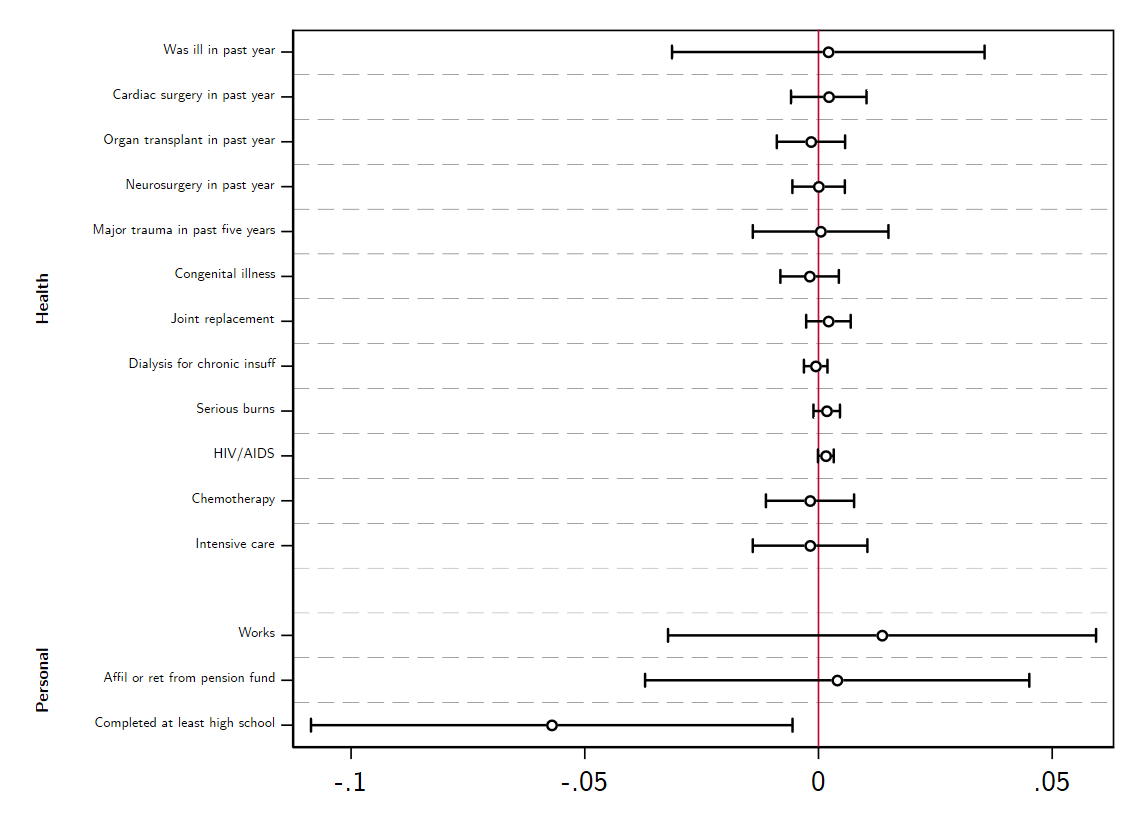
\includegraphics{Graphs/balanceRD_final_F55.png}
    }
    \vfill
    \centering
    \hyperlink{balance}{\beamergotobutton{Back}}
\end{frame}


%% Consultations
\begin{frame}[label=f55_consul_cum]{Health results}
    \centering
    \resizebox{0.8\textwidth}{!}{
      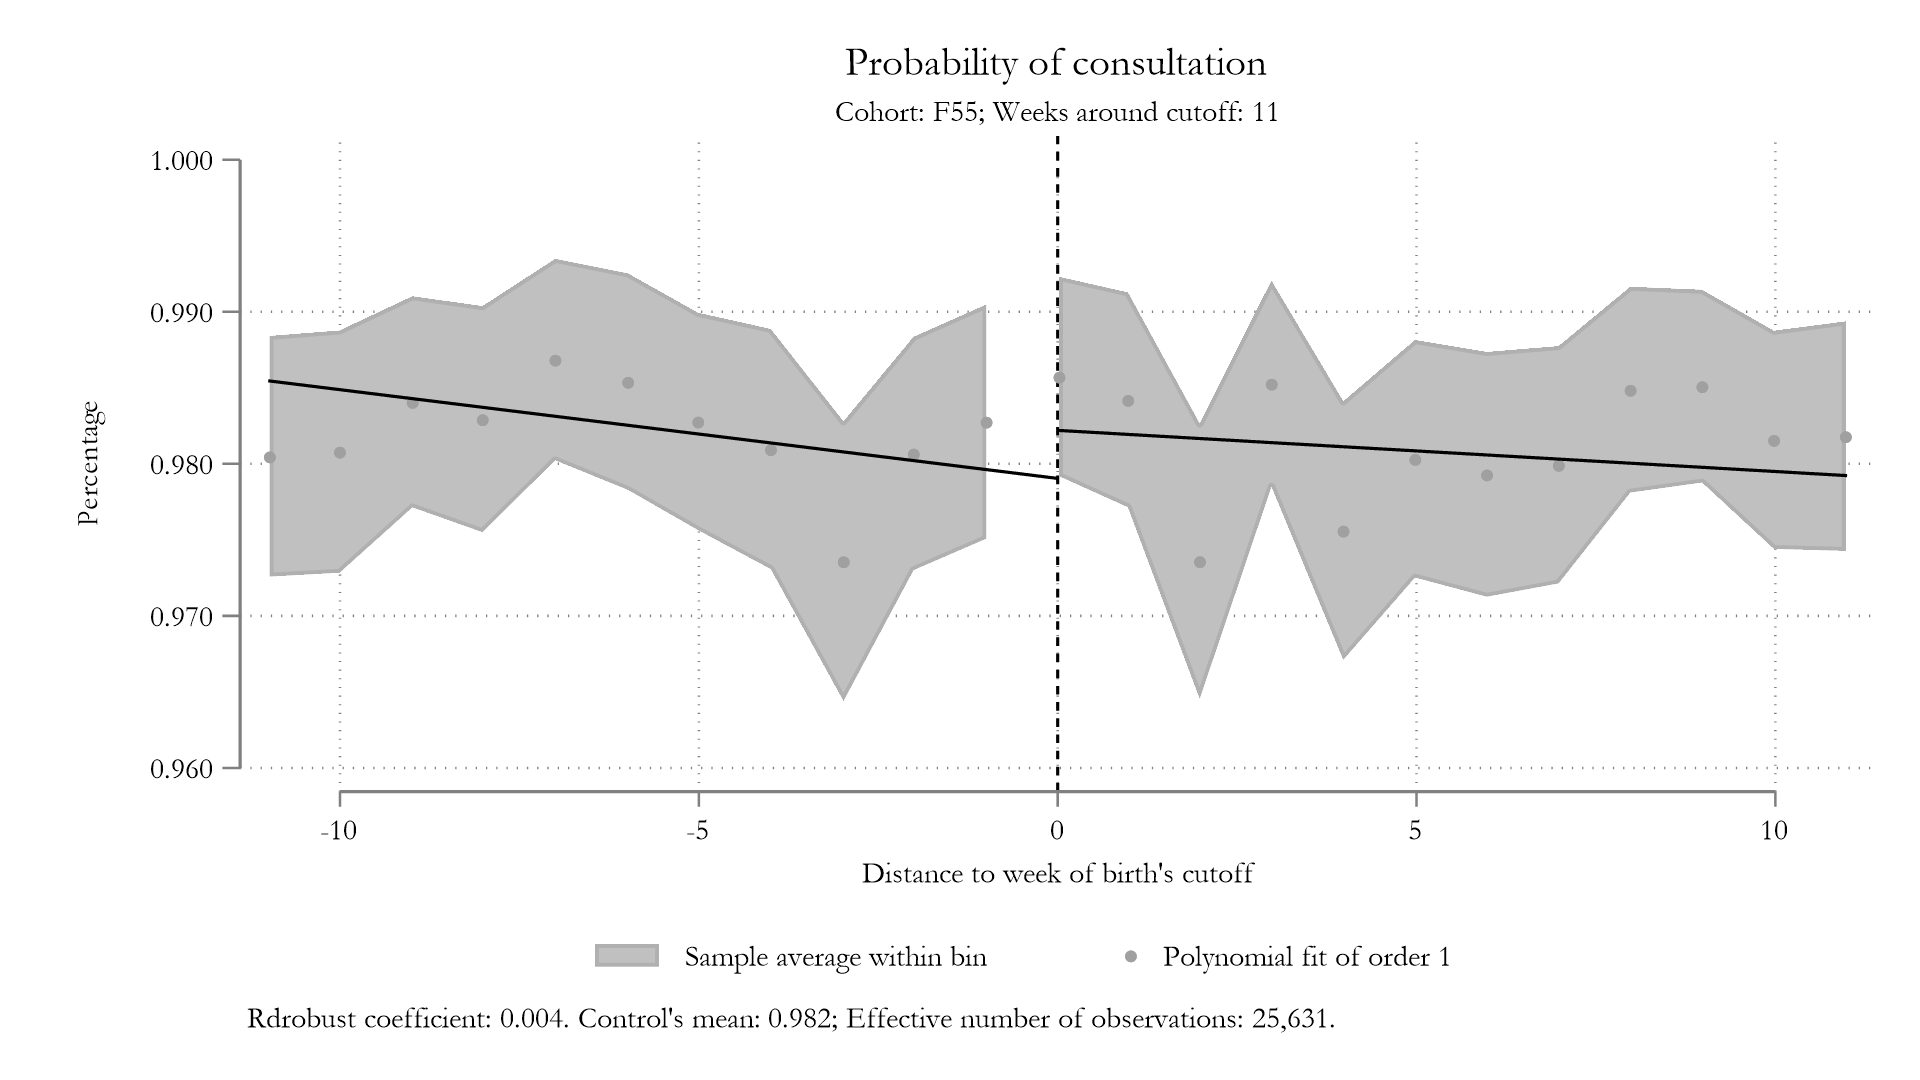
\includegraphics{Graphs/cumulative/consul_F55_11.png}
    }
    \vfill
    \centering
    \hyperlink{f55_consul}{\beamergotobutton{Back}}
\end{frame}

\begin{frame}[label=m50_consul_cum]{Health results}
    \centering
    \resizebox{0.8\textwidth}{!}{
      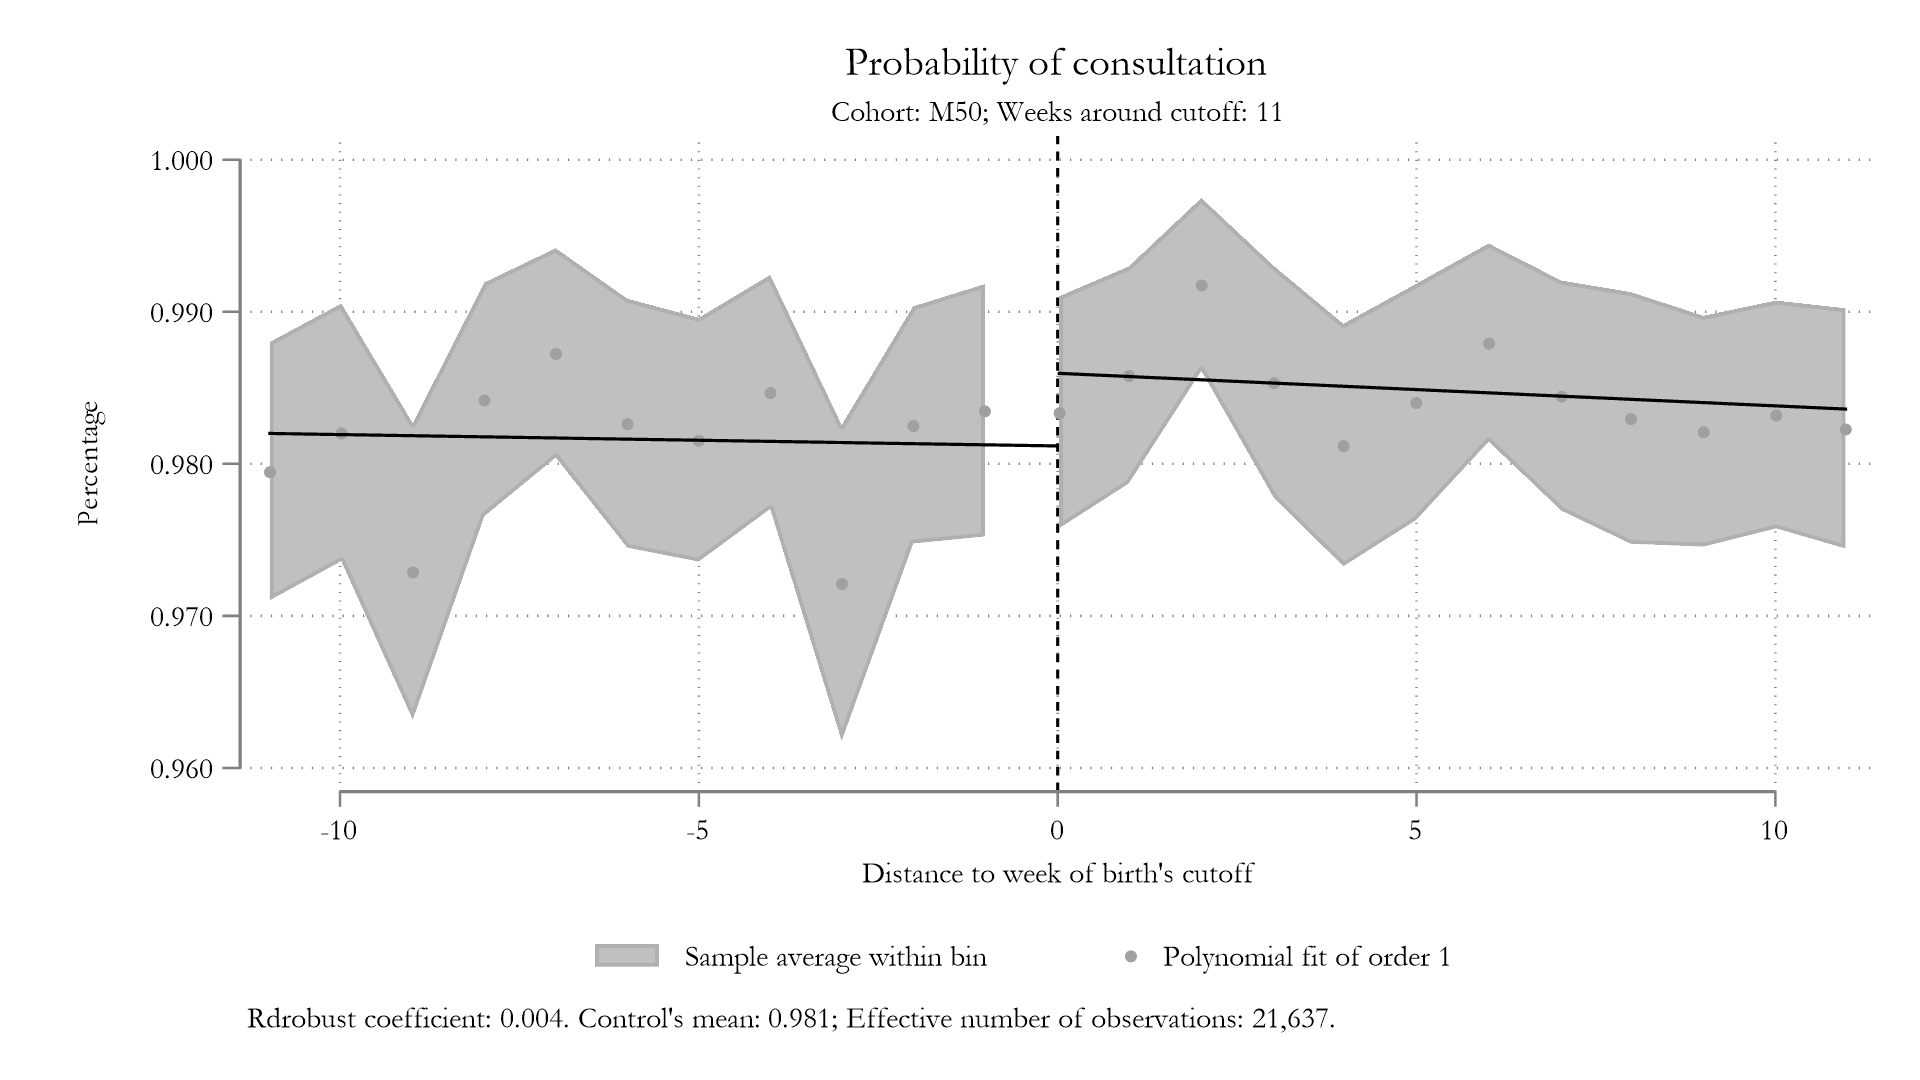
\includegraphics{Graphs/cumulative/consul_M50_11.png}
    }
    \vfill
    \centering
    \hyperlink{m50_consul}{\beamergotobutton{Back}}
\end{frame}

\begin{frame}[label=f55_nroconsul]{Health results}
    \centering
    \resizebox{0.8\textwidth}{!}{
      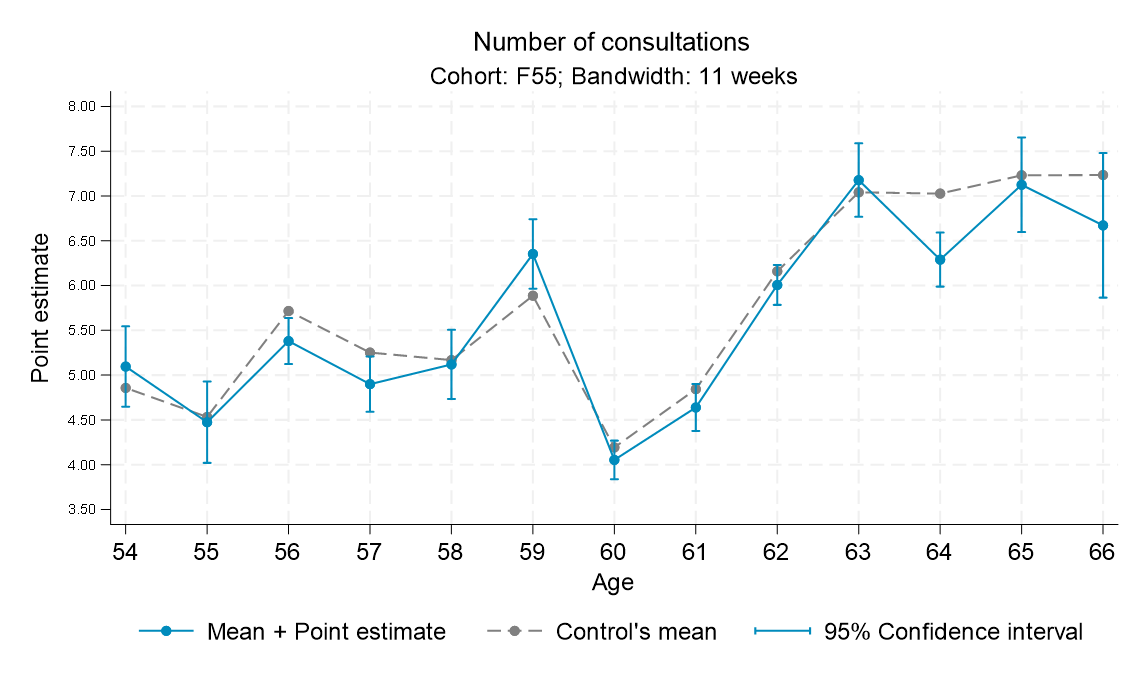
\includegraphics{Graphs/age/nro_consultas_F55_11_age.png}
    }
    \vfill
    \centering
    \hyperlink{f55_consul}{\beamergotobutton{Back to main}}
    \hyperlink{f55_nroconsul_cum}{\beamergotobutton{See cumulative}}
\end{frame}

\begin{frame}[label=m50_nroconsul]{Health results}
    \centering
    \resizebox{0.8\textwidth}{!}{
      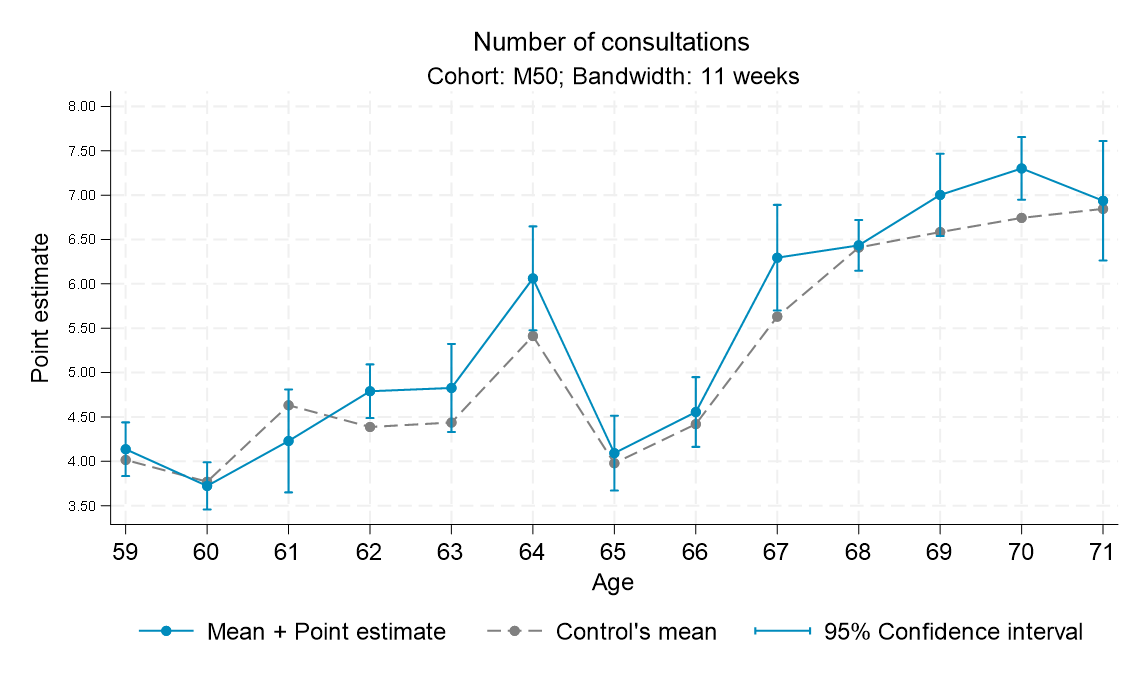
\includegraphics{Graphs/age/nro_consultas_M50_11_age.png}
    }
    \vfill
    \centering
    \hyperlink{m50_consul}{\beamergotobutton{Back to main}}
    \hyperlink{m50_nroconsul_cum}{\beamergotobutton{See cumulative}}
\end{frame}

\begin{frame}[label=f55_nroconsul_cum]{Health results}
    \centering
    \resizebox{0.8\textwidth}{!}{
      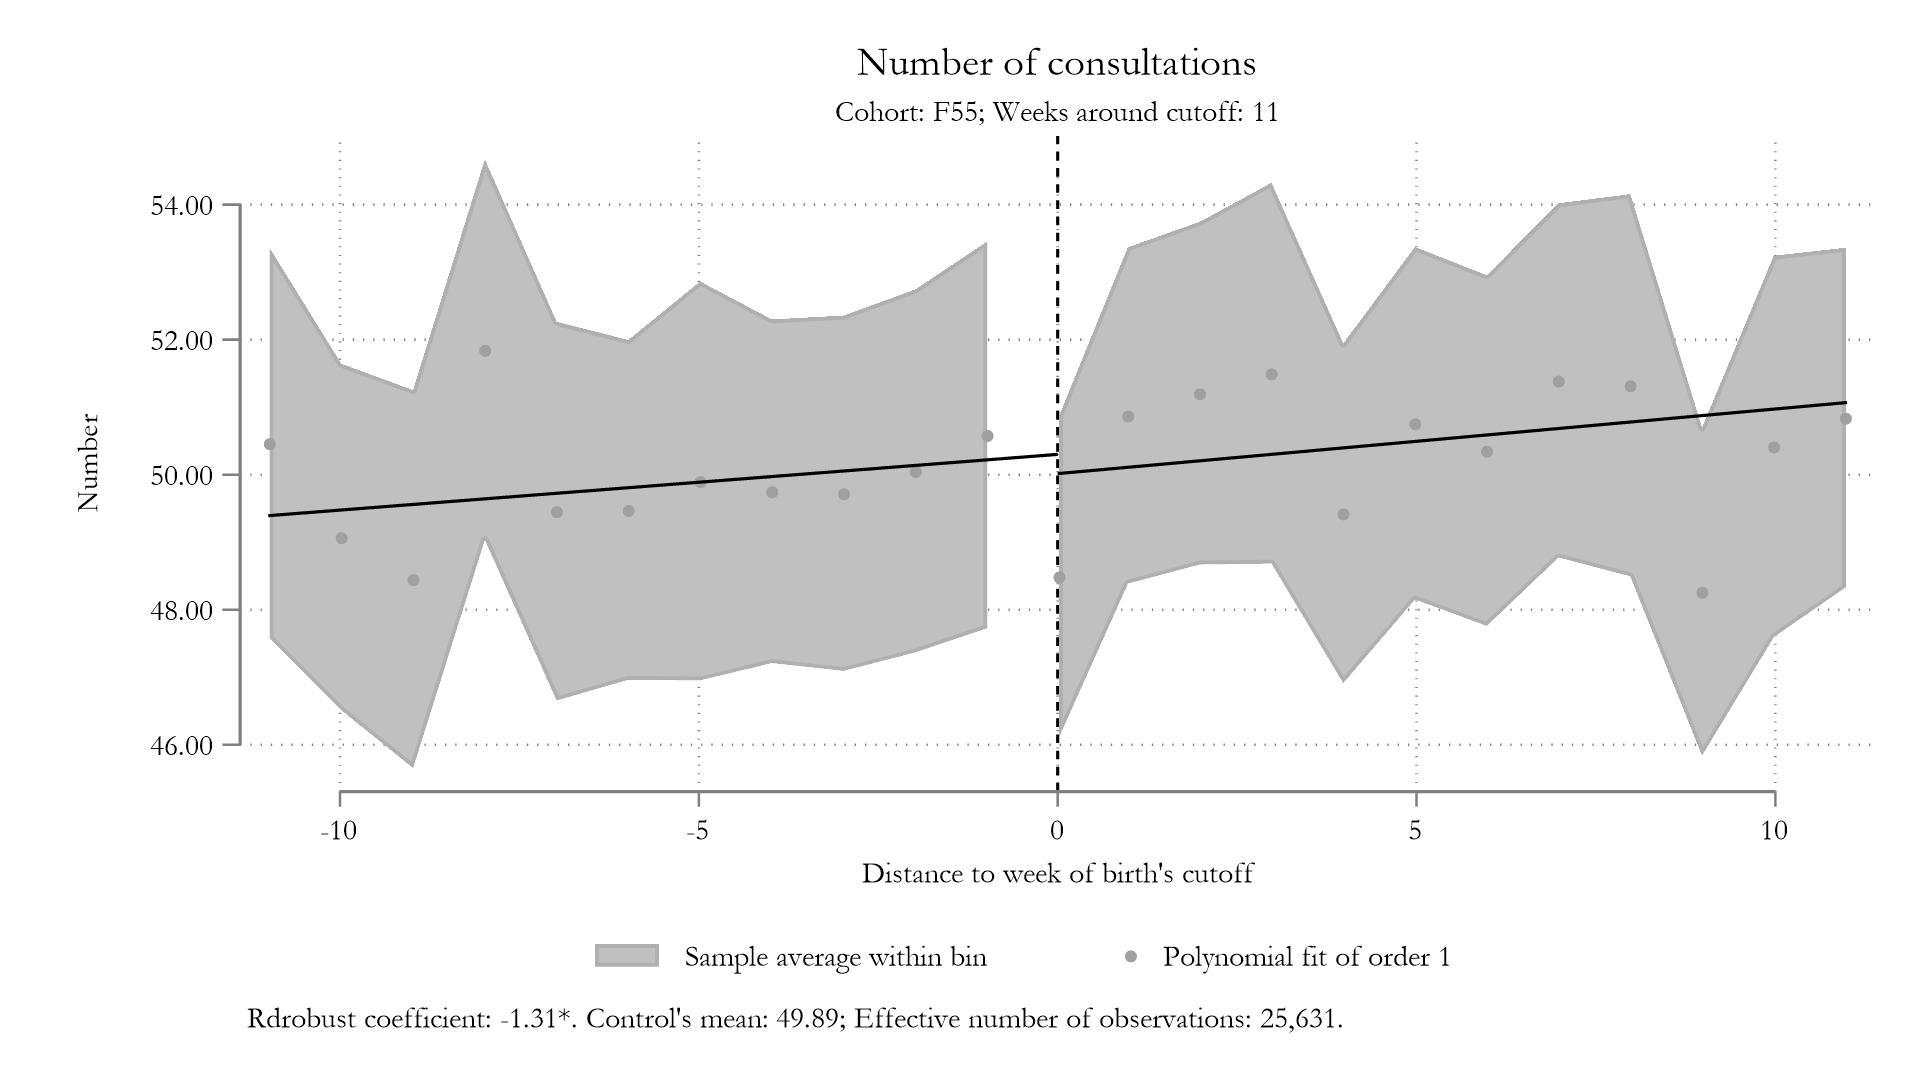
\includegraphics{Graphs/cumulative/nro_consultas_F55_11.png}
    }
    \vfill
    \centering
    \hyperlink{f55_consul}{\beamergotobutton{Back to main}}
\end{frame}

\begin{frame}[label=m50_nroconsul_cum]{Health results}
    \centering
    \resizebox{0.8\textwidth}{!}{
      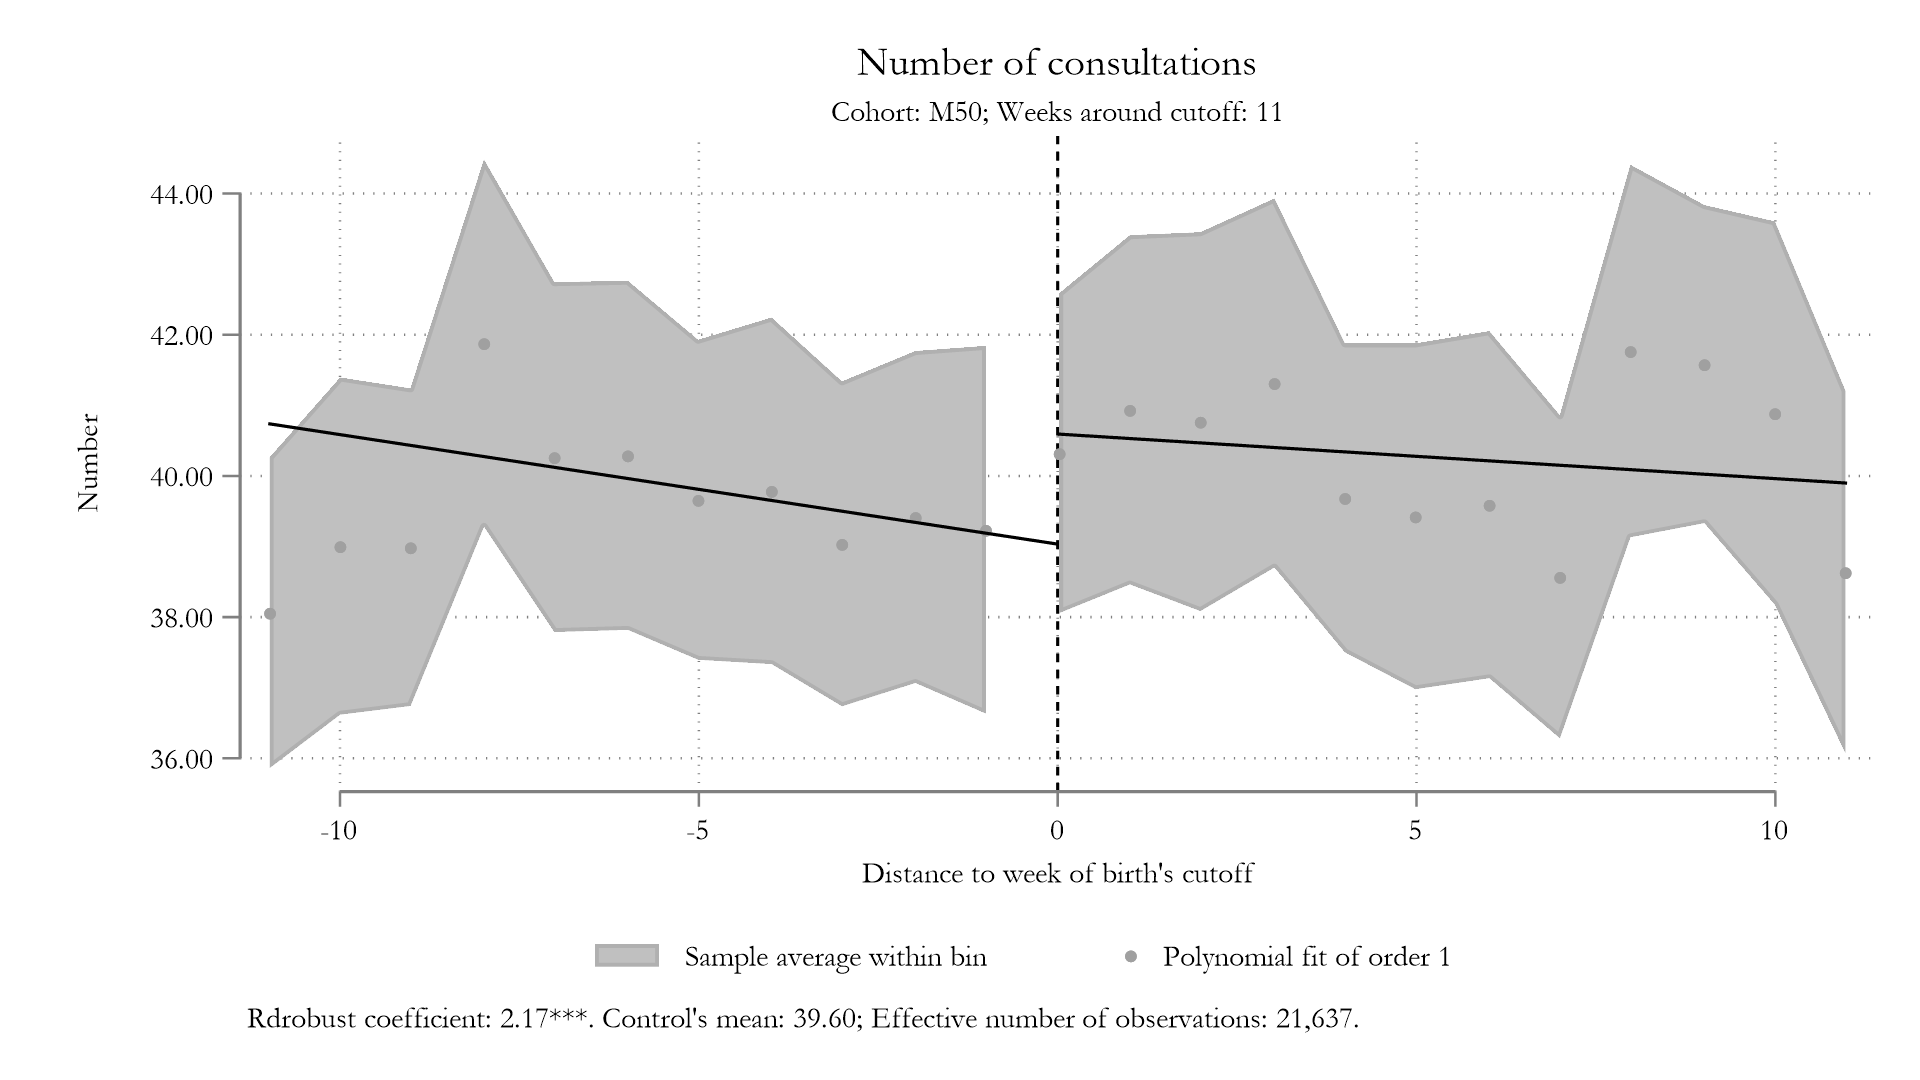
\includegraphics{Graphs/cumulative/nro_consultas_M50_11.png}
    }
    \vfill
    \centering
    \hyperlink{m50_consul}{\beamergotobutton{Back to main}}
\end{frame}


%%% Hosp
\begin{frame}[label=f55_hosp_cum]{Health results}
    \centering
    \resizebox{0.8\textwidth}{!}{
      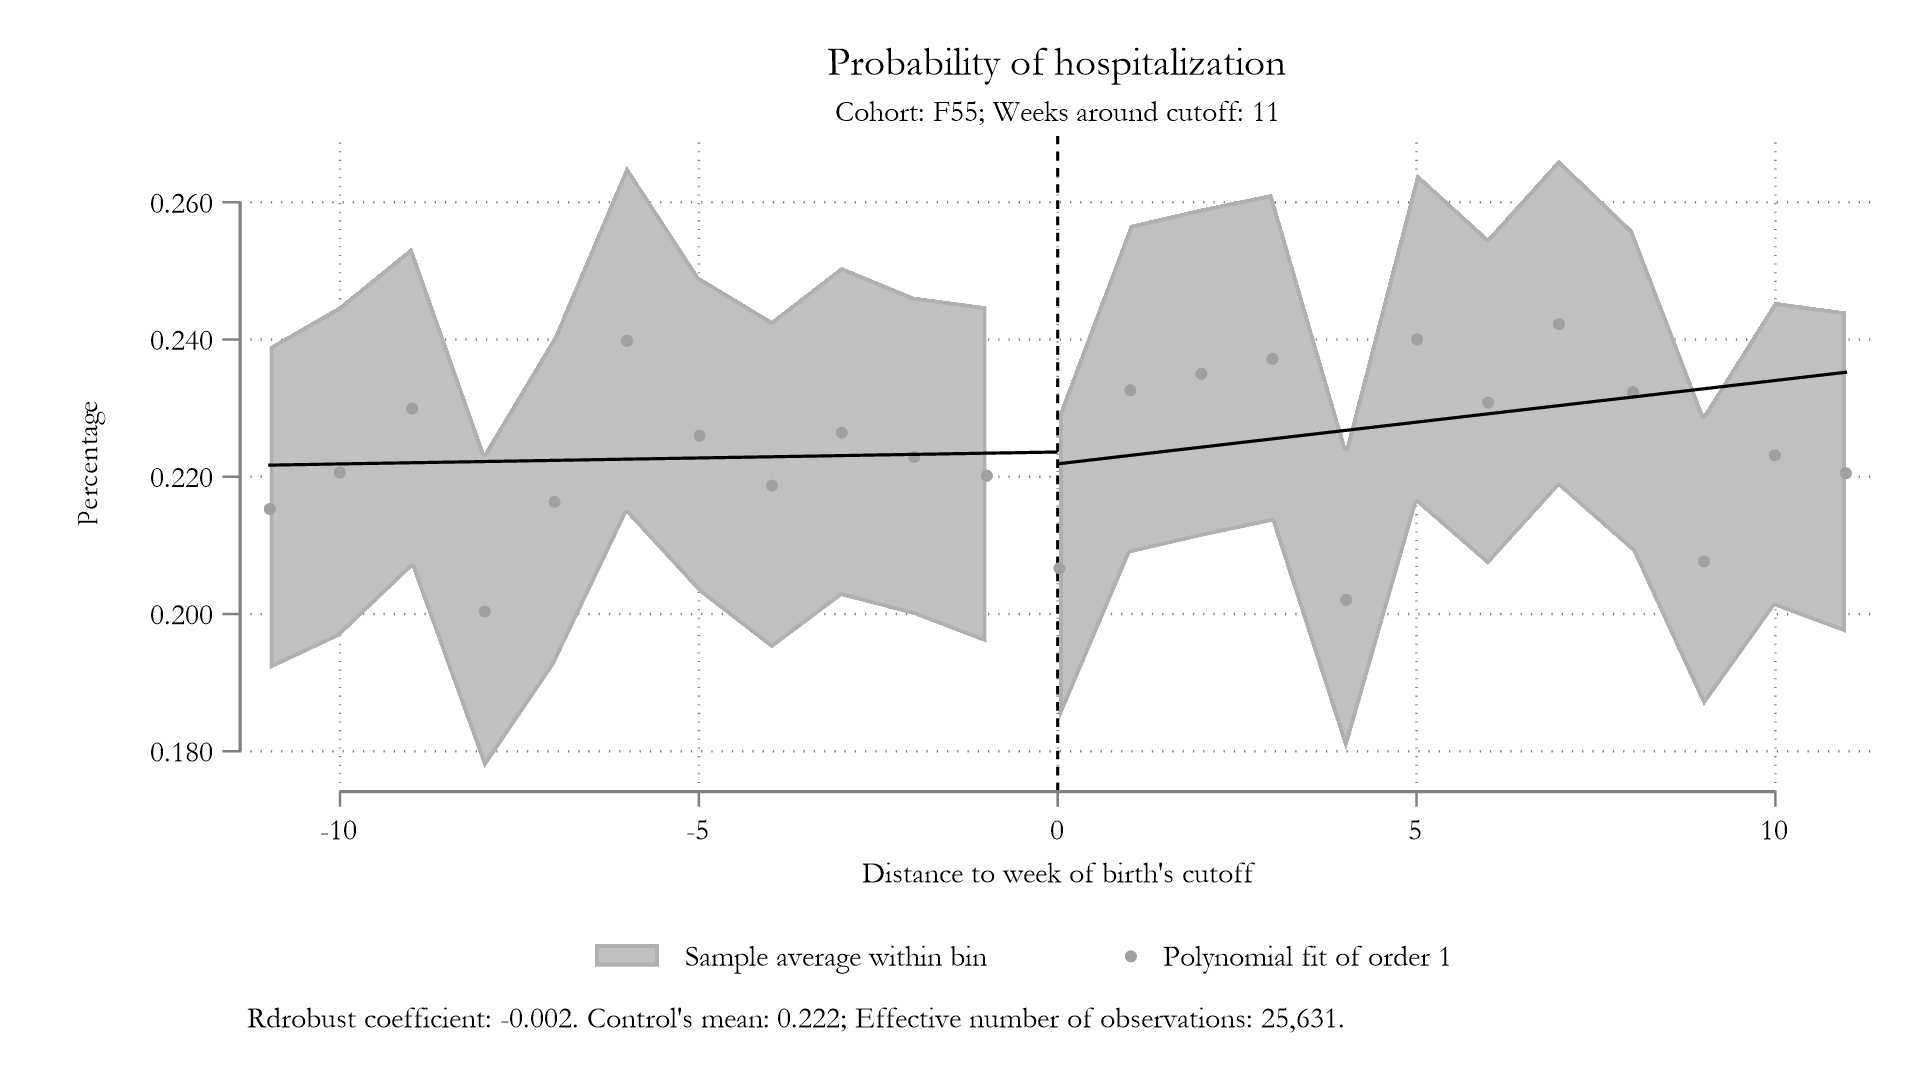
\includegraphics{Graphs/cumulative/hosp_F55_11.png}
    }
    \vfill
    \centering
    \hyperlink{f55_hosp}{\beamergotobutton{Back}}
\end{frame}

\begin{frame}[label=m50_hosp_cum]{Health results}
    \centering
    \resizebox{0.8\textwidth}{!}{
      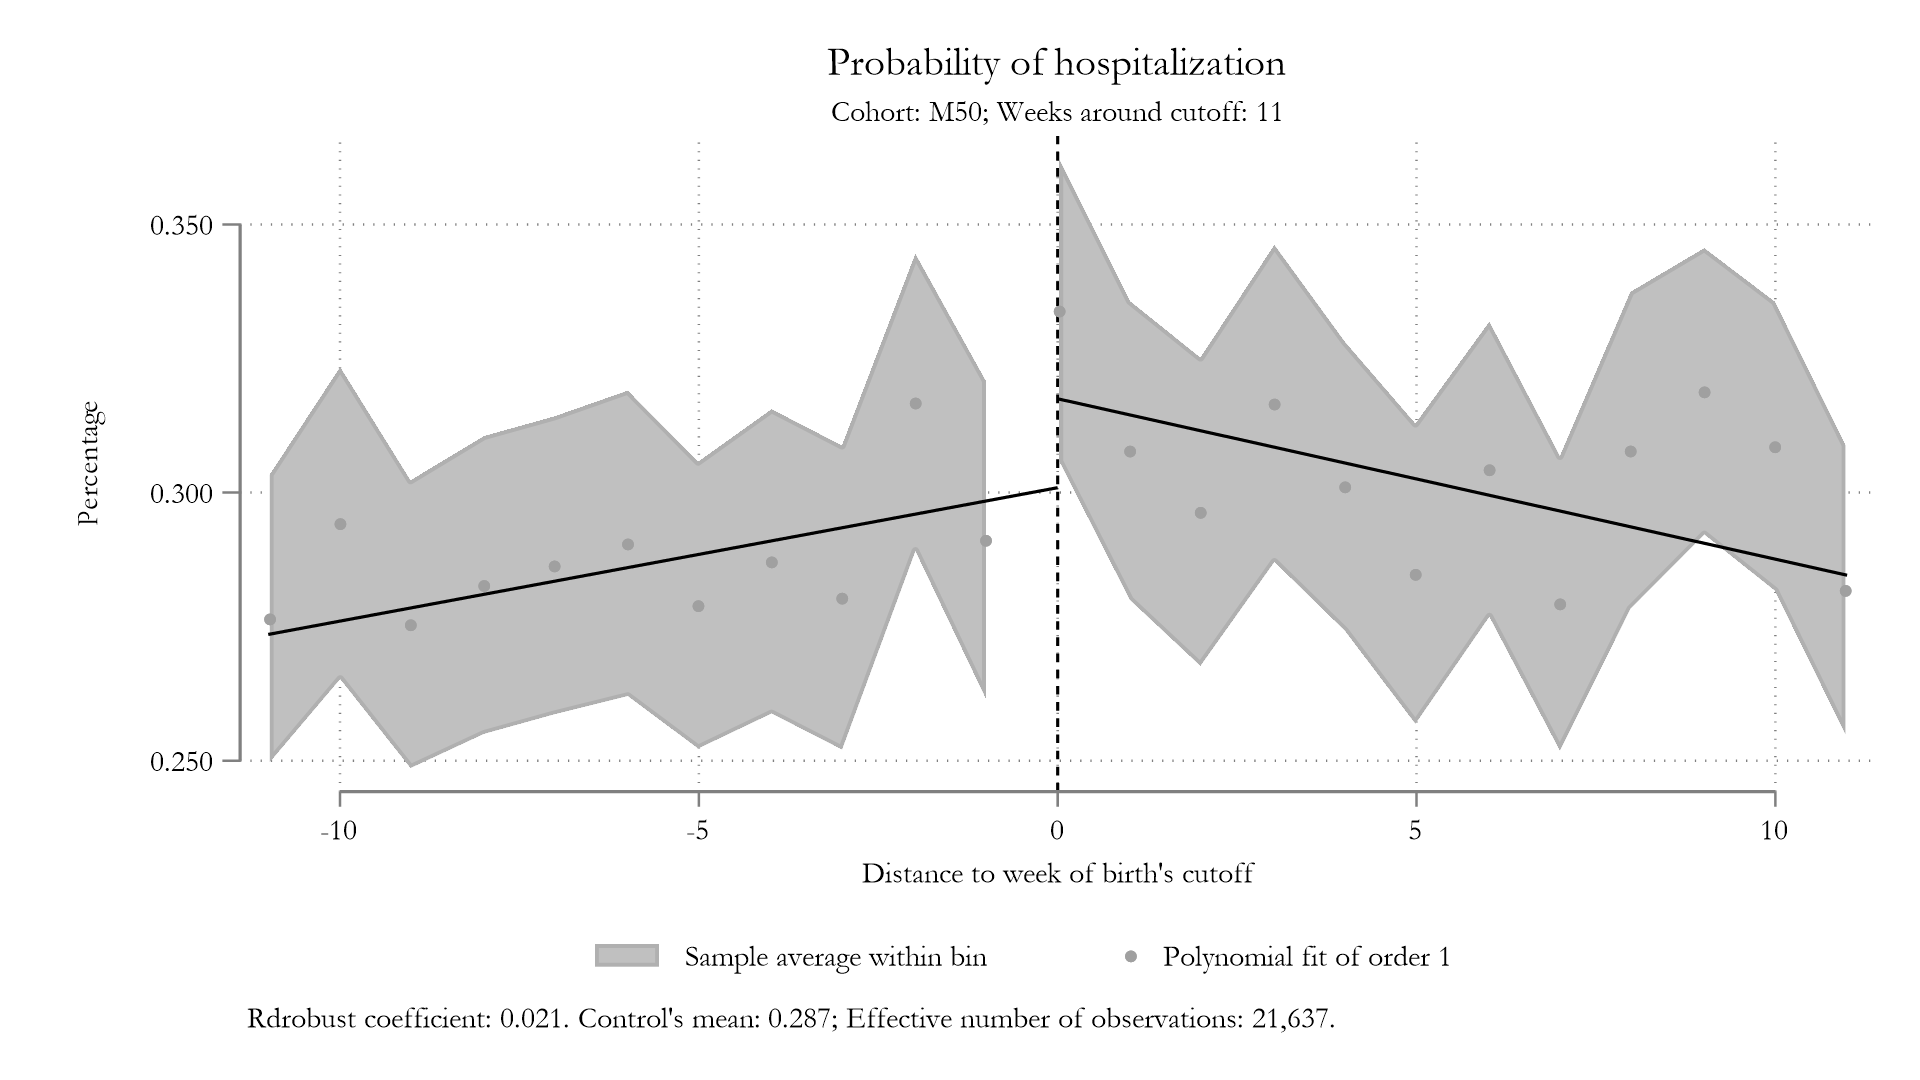
\includegraphics{Graphs/cumulative/hosp_M50_11.png}
    }
    \vfill
    \centering
    \hyperlink{m50_hosp}{\beamergotobutton{Back}}
\end{frame}

\begin{frame}[label=f55_nrohosp]{Health results}
    \centering
    \resizebox{0.8\textwidth}{!}{
      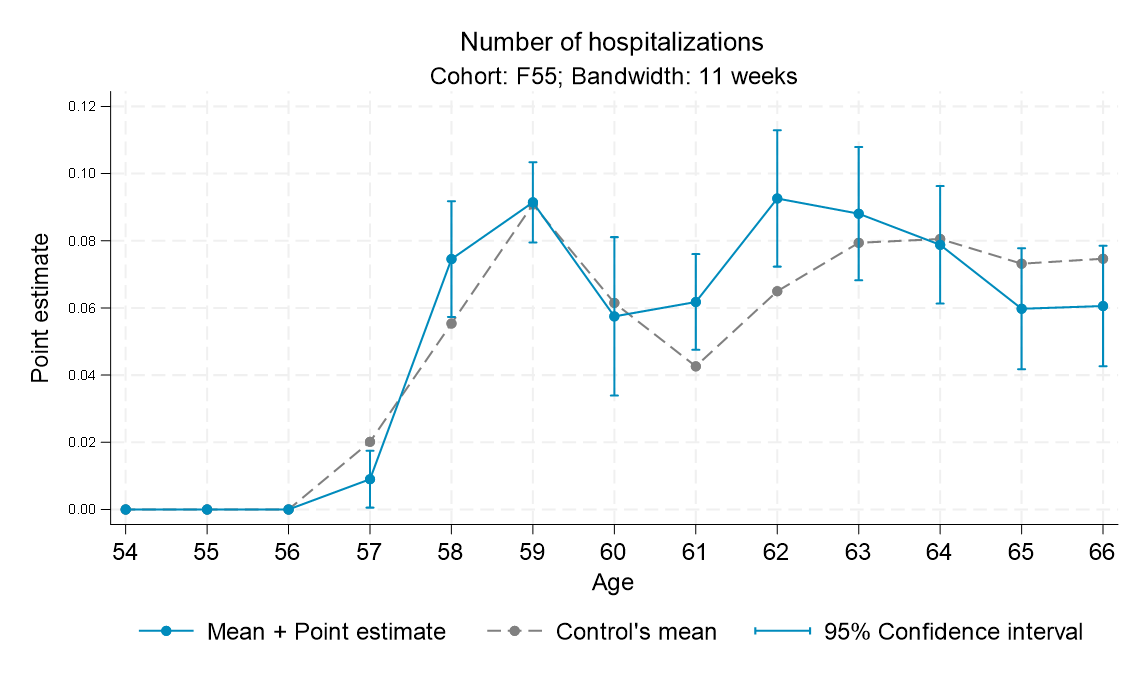
\includegraphics{Graphs/age/nro_Hospitalizacion_F55_11_age.png}
    }
    \vfill
    \centering
    \hyperlink{f55_hosp}{\beamergotobutton{Back to main}}
    \hyperlink{f55_nrohosp_cum}{\beamergotobutton{See cumulative}}
\end{frame}

\begin{frame}[label=m50_nrohosp]{Health results}
    \centering
    \resizebox{0.8\textwidth}{!}{
      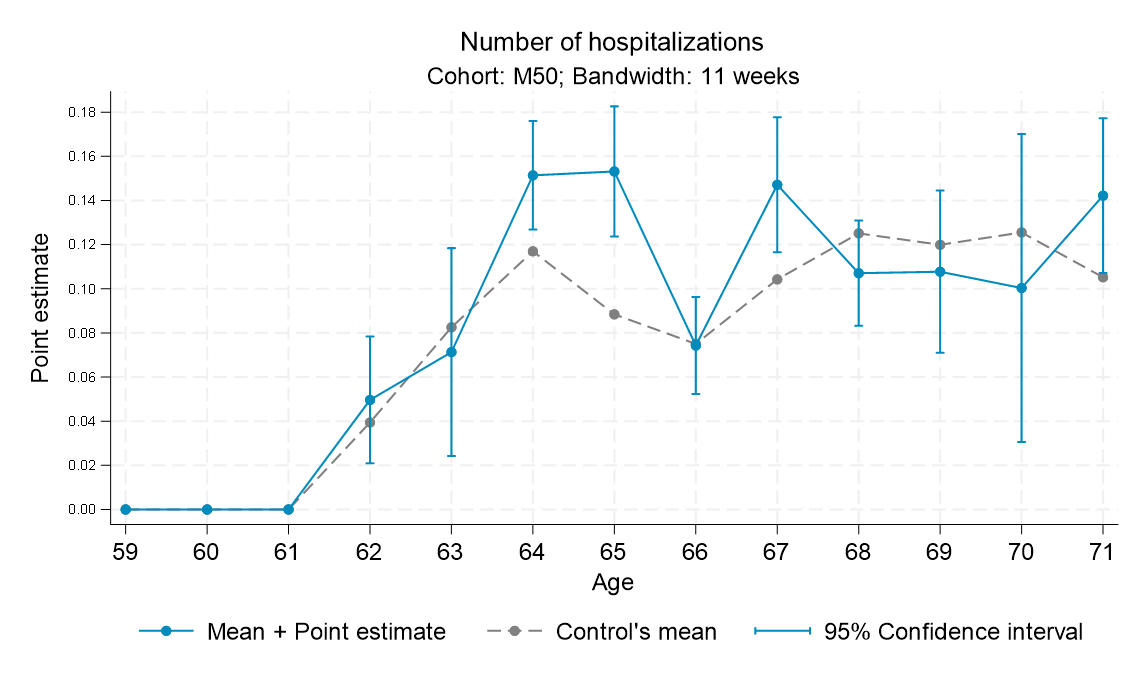
\includegraphics{Graphs/age/nro_Hospitalizacion_M50_11_age.png}
    }
    \vfill
    \centering
    \hyperlink{m50_hosp}{\beamergotobutton{Back to main}}
    \hyperlink{m50_nrohosp_cum}{\beamergotobutton{See cumulative}}
\end{frame}

\begin{frame}[label=f55_nrohosp_cum]{Health results}
    \centering
    \resizebox{0.8\textwidth}{!}{
      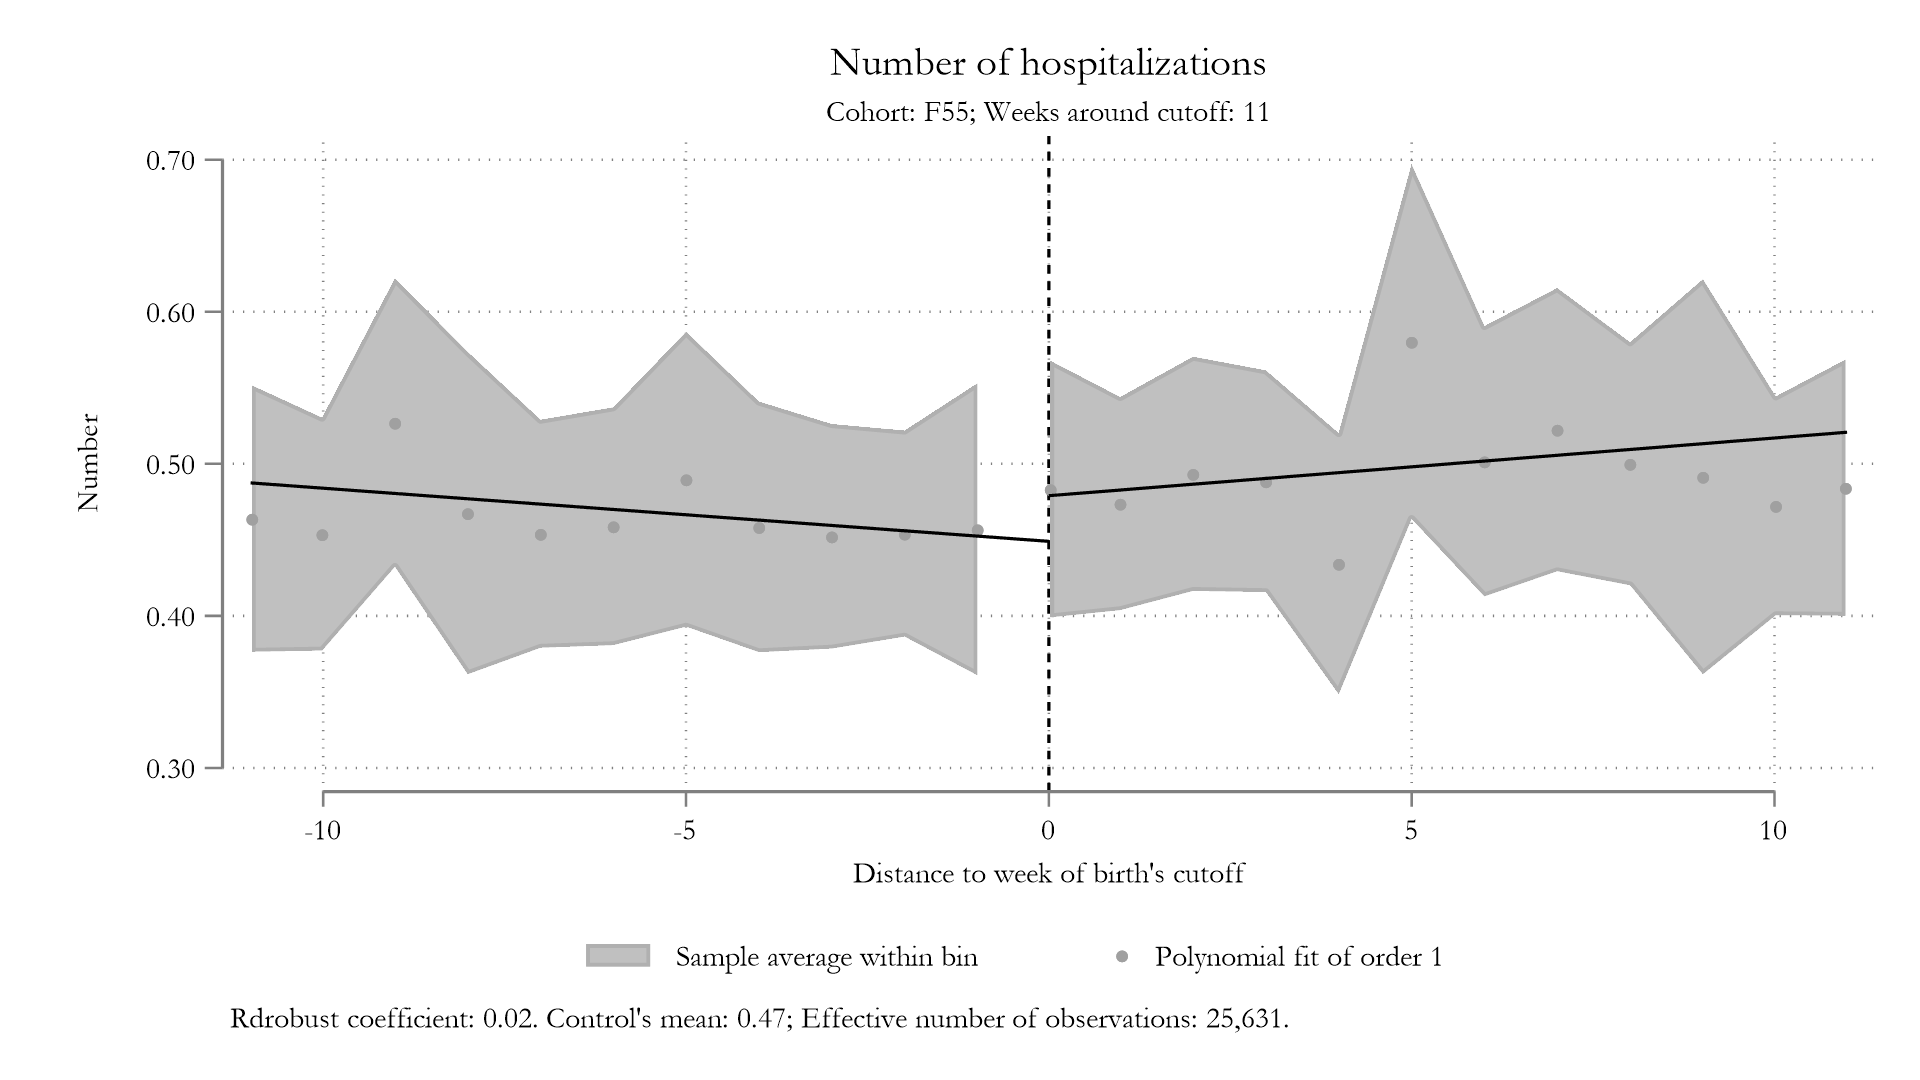
\includegraphics{Graphs/cumulative/nro_Hospitalizacion_F55_11.png}
    }
    \vfill
    \centering
    \hyperlink{f55_hosp}{\beamergotobutton{Back to main}}
\end{frame}

\begin{frame}[label=m50_nrohosp_cum]{Health results}
    \centering
    \resizebox{0.8\textwidth}{!}{
      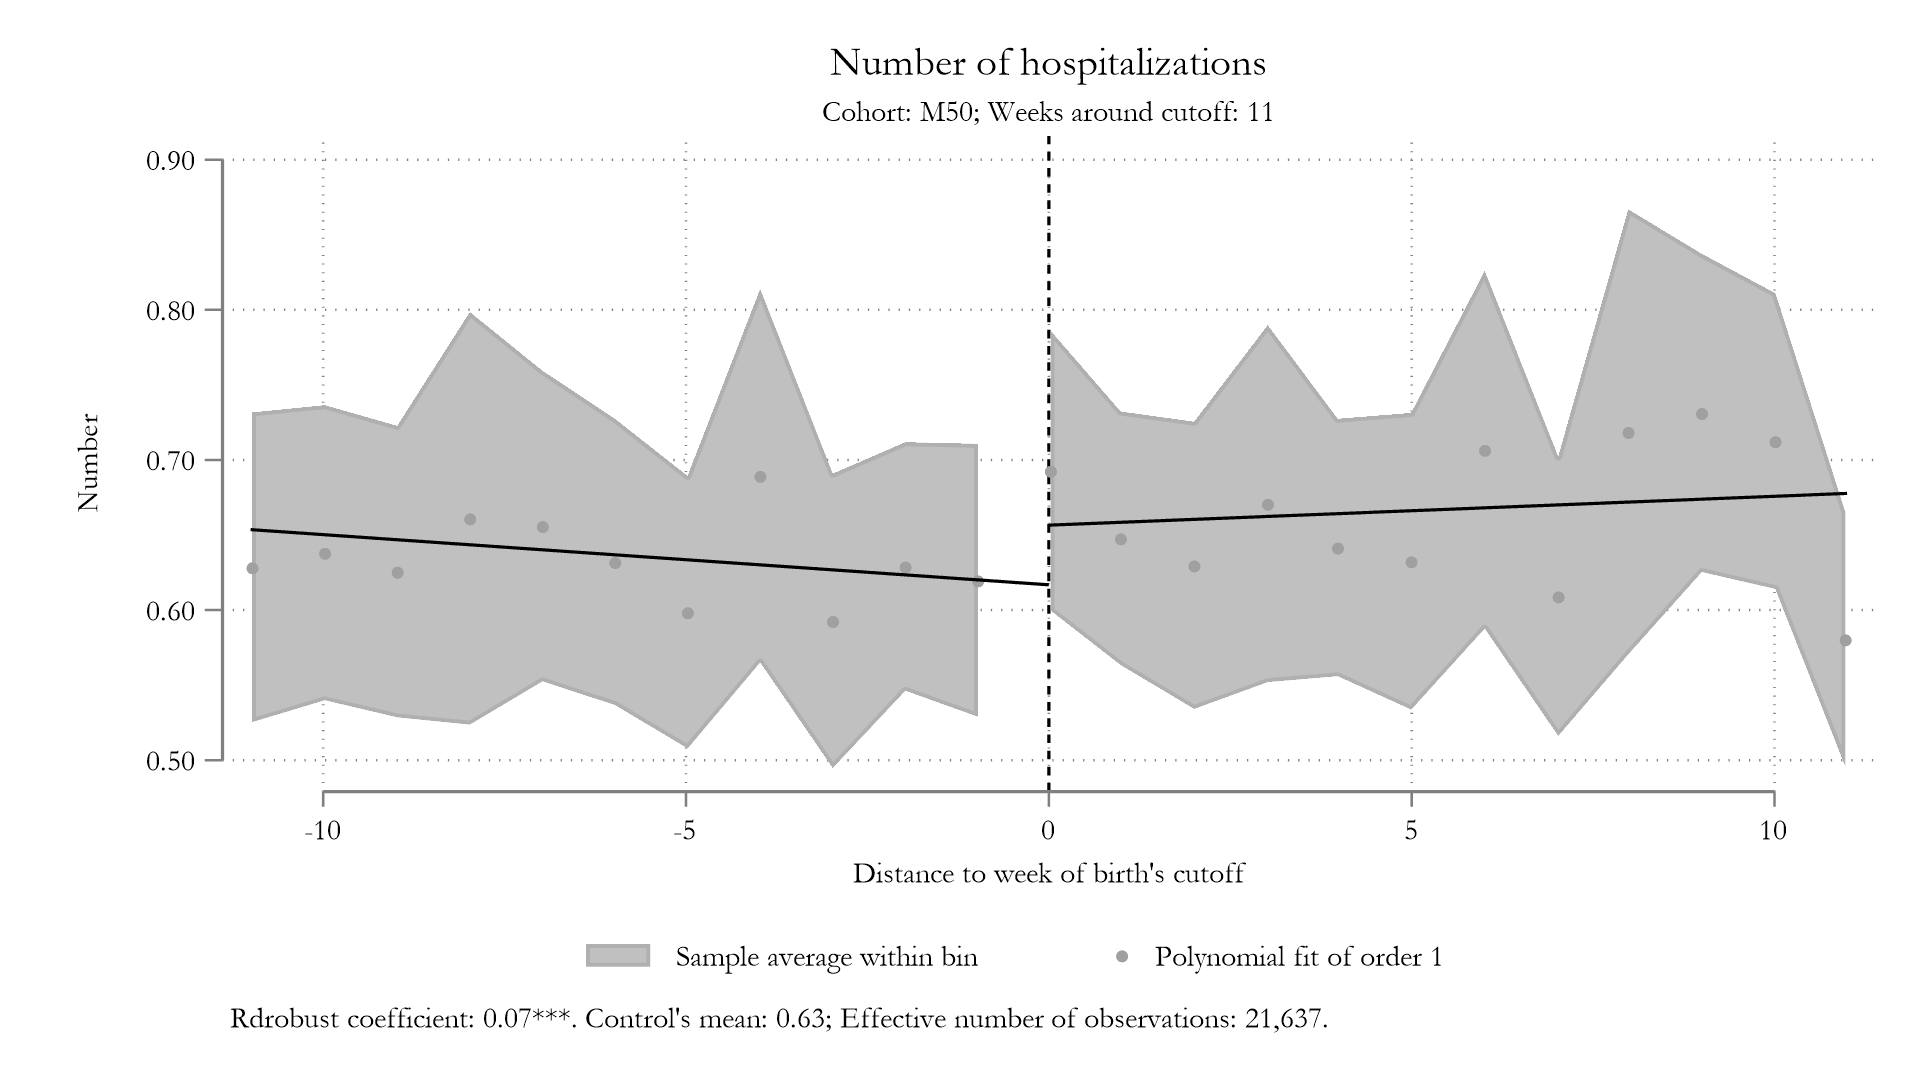
\includegraphics{Graphs/cumulative/nro_Hospitalizacion_M50_11.png}
    }
    \vfill
    \centering
    \hyperlink{m50_hosp}{\beamergotobutton{Back to main}}
\end{frame}


%% Cardio

\begin{frame}[label=f55_cardio_cum]{Health results}
    \centering
    \resizebox{0.8\textwidth}{!}{
      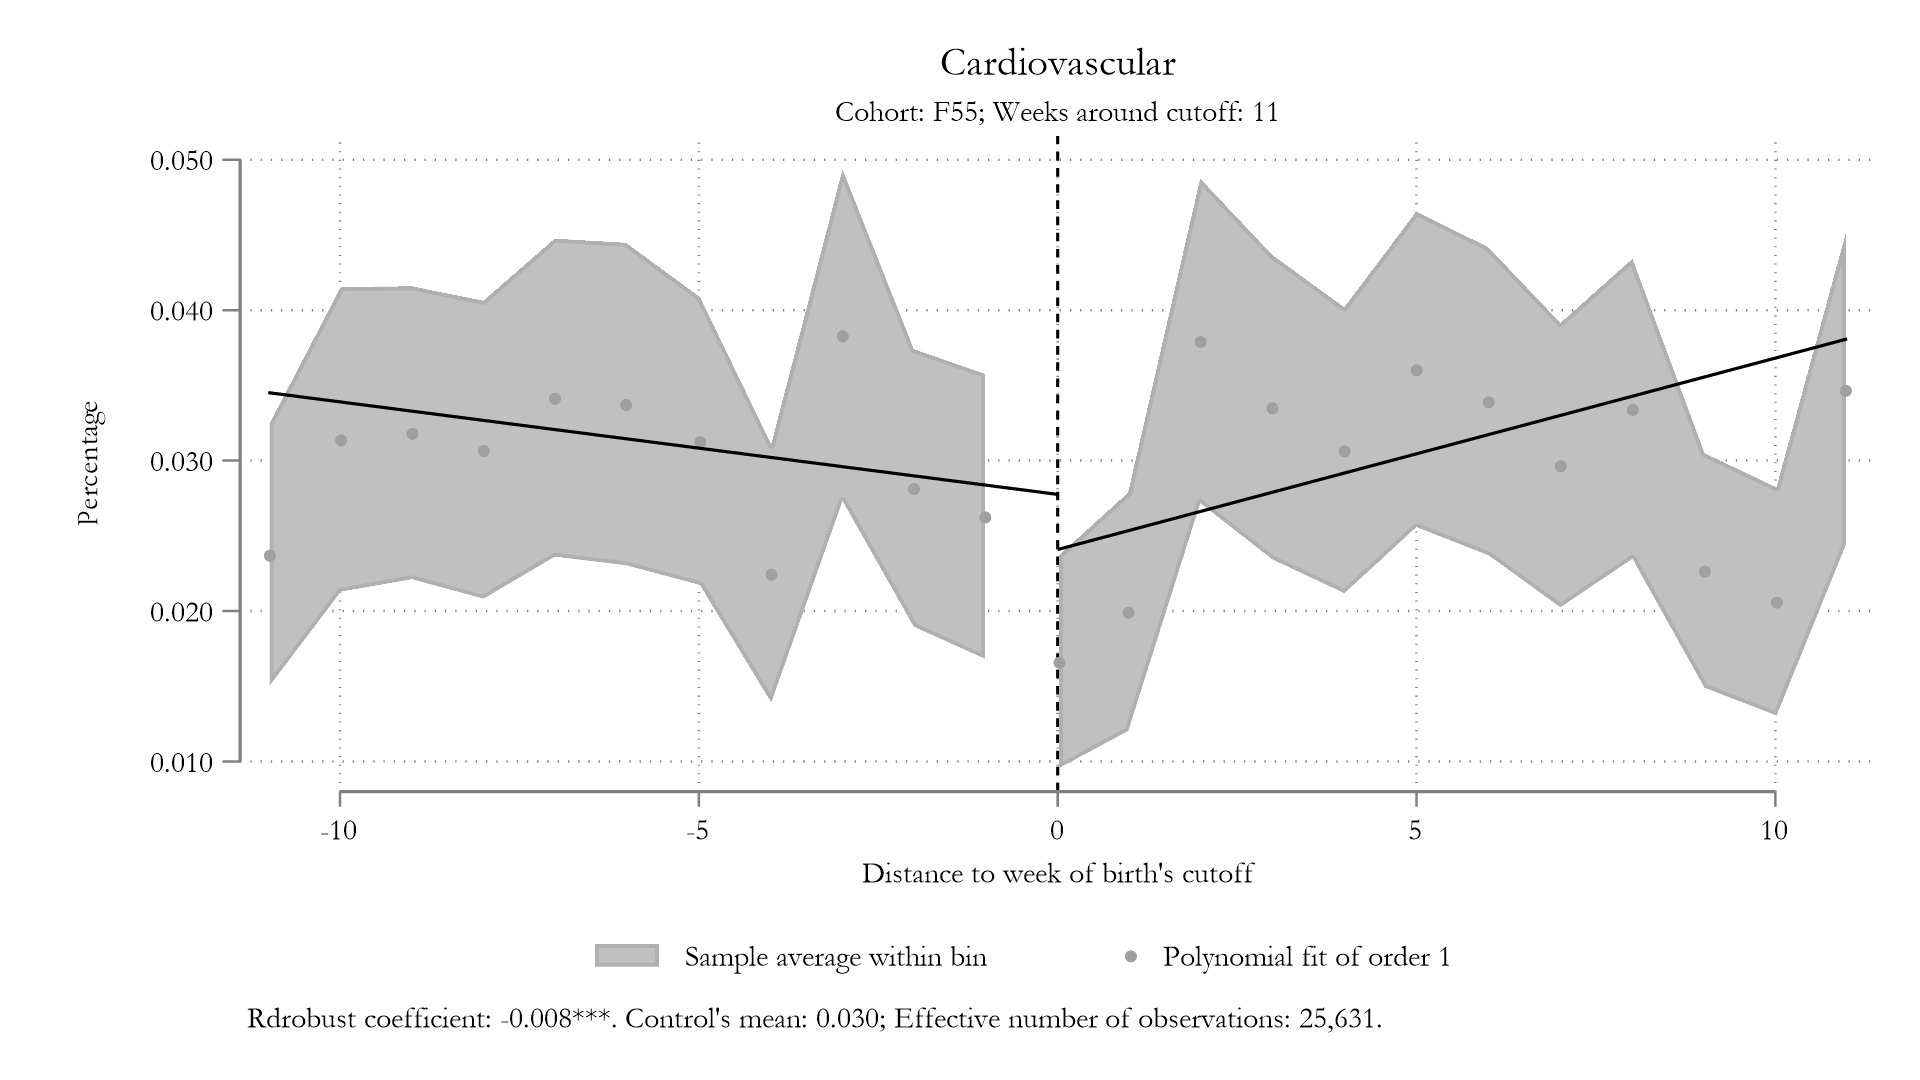
\includegraphics{Graphs/cumulative/cardiovascular_F55_11.png}
    }
    \vfill
    \centering
    \hyperlink{f55_cardio}{\beamergotobutton{Back}}
\end{frame}

\begin{frame}[label=m50_cardio_cum]{Health results}
    \centering
    \resizebox{0.8\textwidth}{!}{
      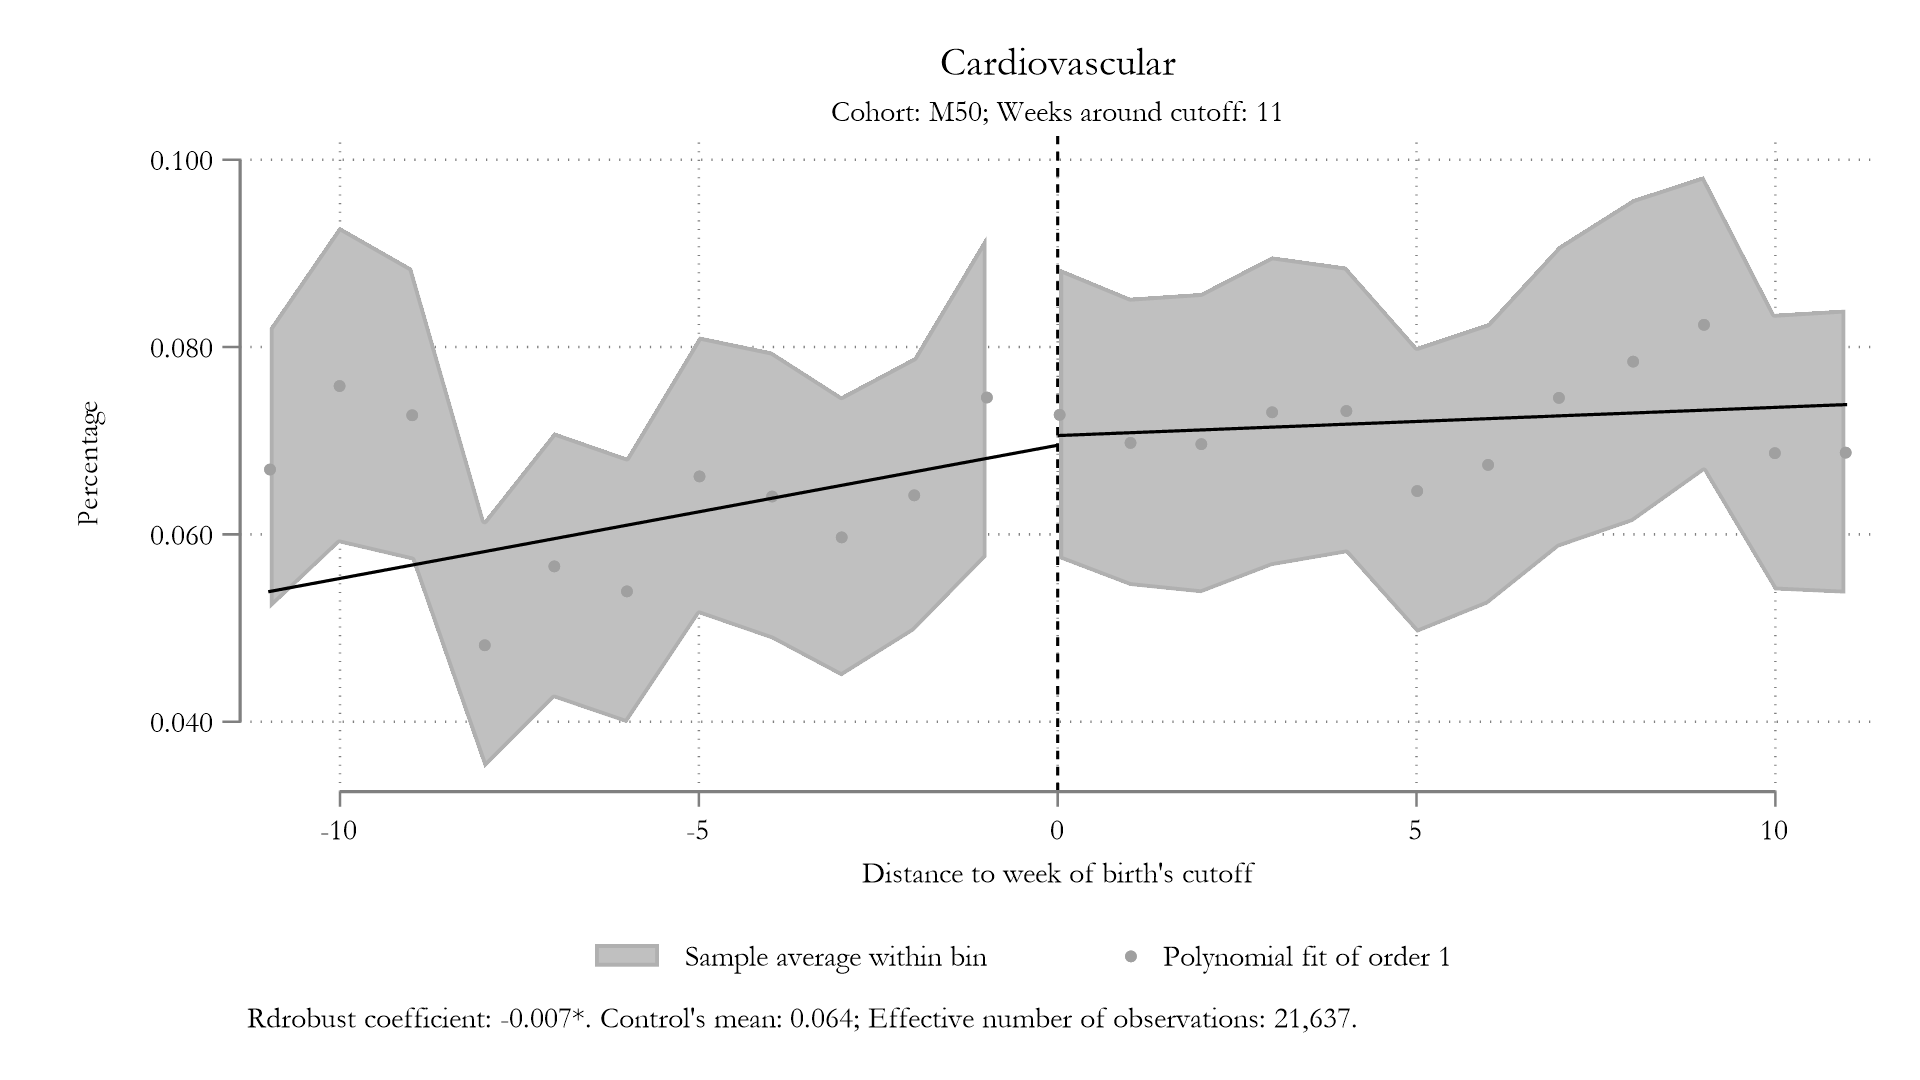
\includegraphics{Graphs/cumulative/cardiovascular_M50_11.png}
    }
    \vfill
    \centering
    \hyperlink{m50_cardio}{\beamergotobutton{Back}}
\end{frame}


%% Infarct

\begin{frame}[label=f55_infarct_cum]{Health results}
    \centering
    \resizebox{0.8\textwidth}{!}{
      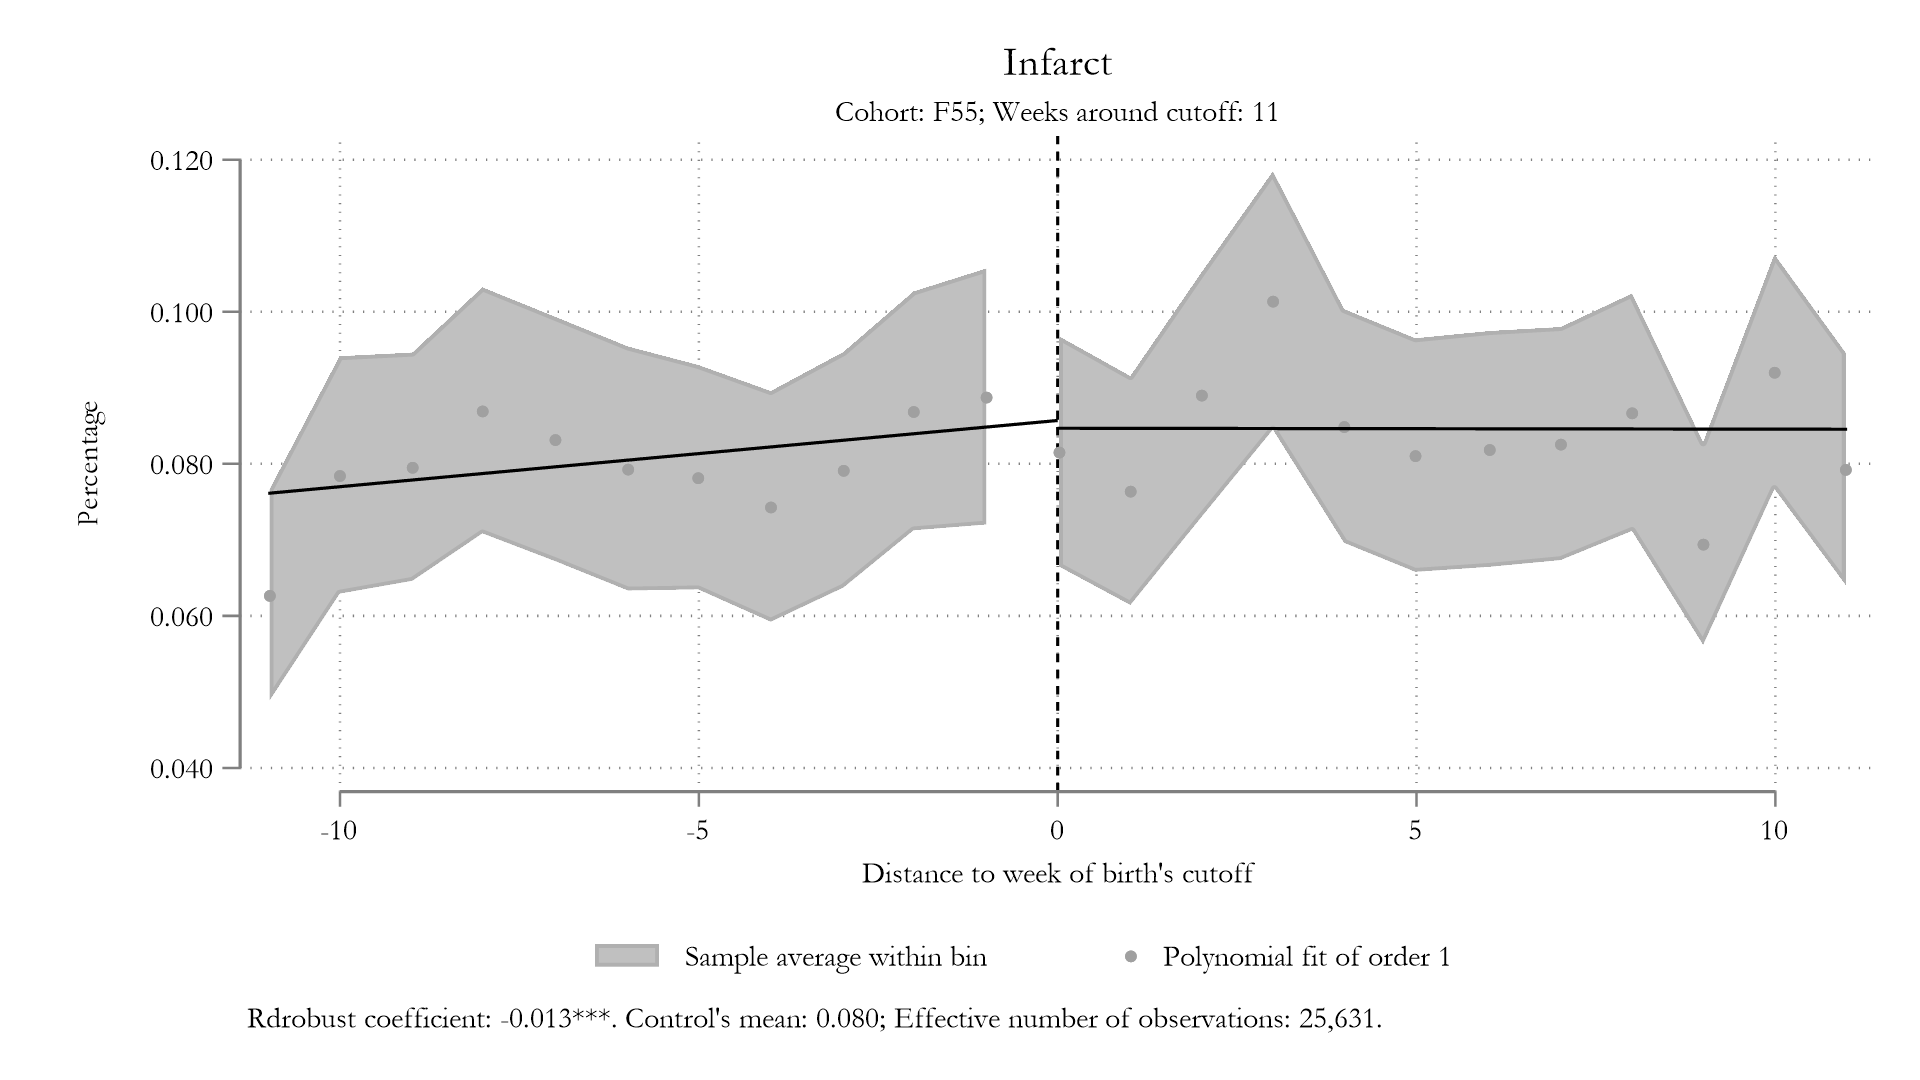
\includegraphics{Graphs/cumulative/infarct_F55_11.png}
    }
    \vfill
    \centering
    \hyperlink{f55_infarct}{\beamergotobutton{Back}}
\end{frame}

\begin{frame}[label=m50_infarct_cum]{Health results}
    \centering
    \resizebox{0.8\textwidth}{!}{
      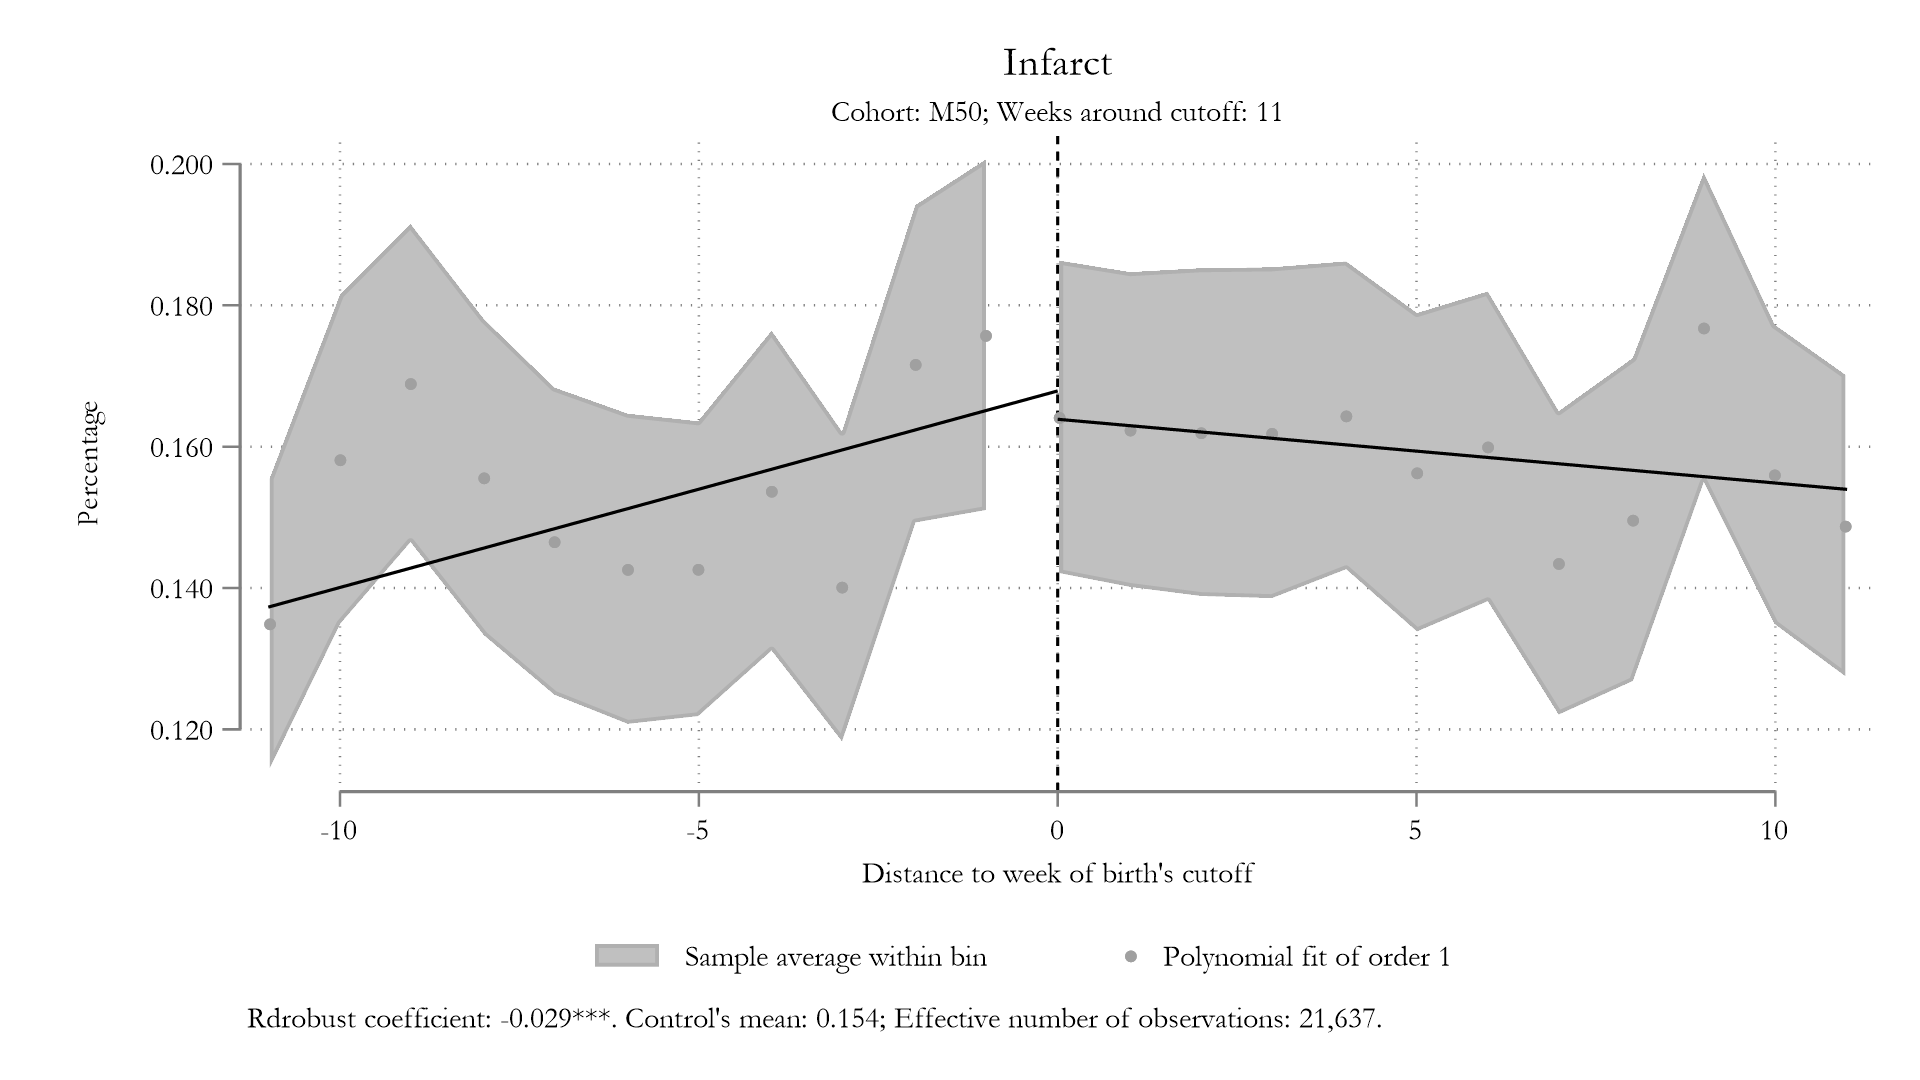
\includegraphics{Graphs/cumulative/infarct_M50_11.png}
    }
    \vfill
    \centering
    \hyperlink{m50_infarct}{\beamergotobutton{Back}}
\end{frame}


%% Stress
\begin{frame}[label=f55_stress_cum]{Health results}
    \centering
    \resizebox{0.8\textwidth}{!}{
      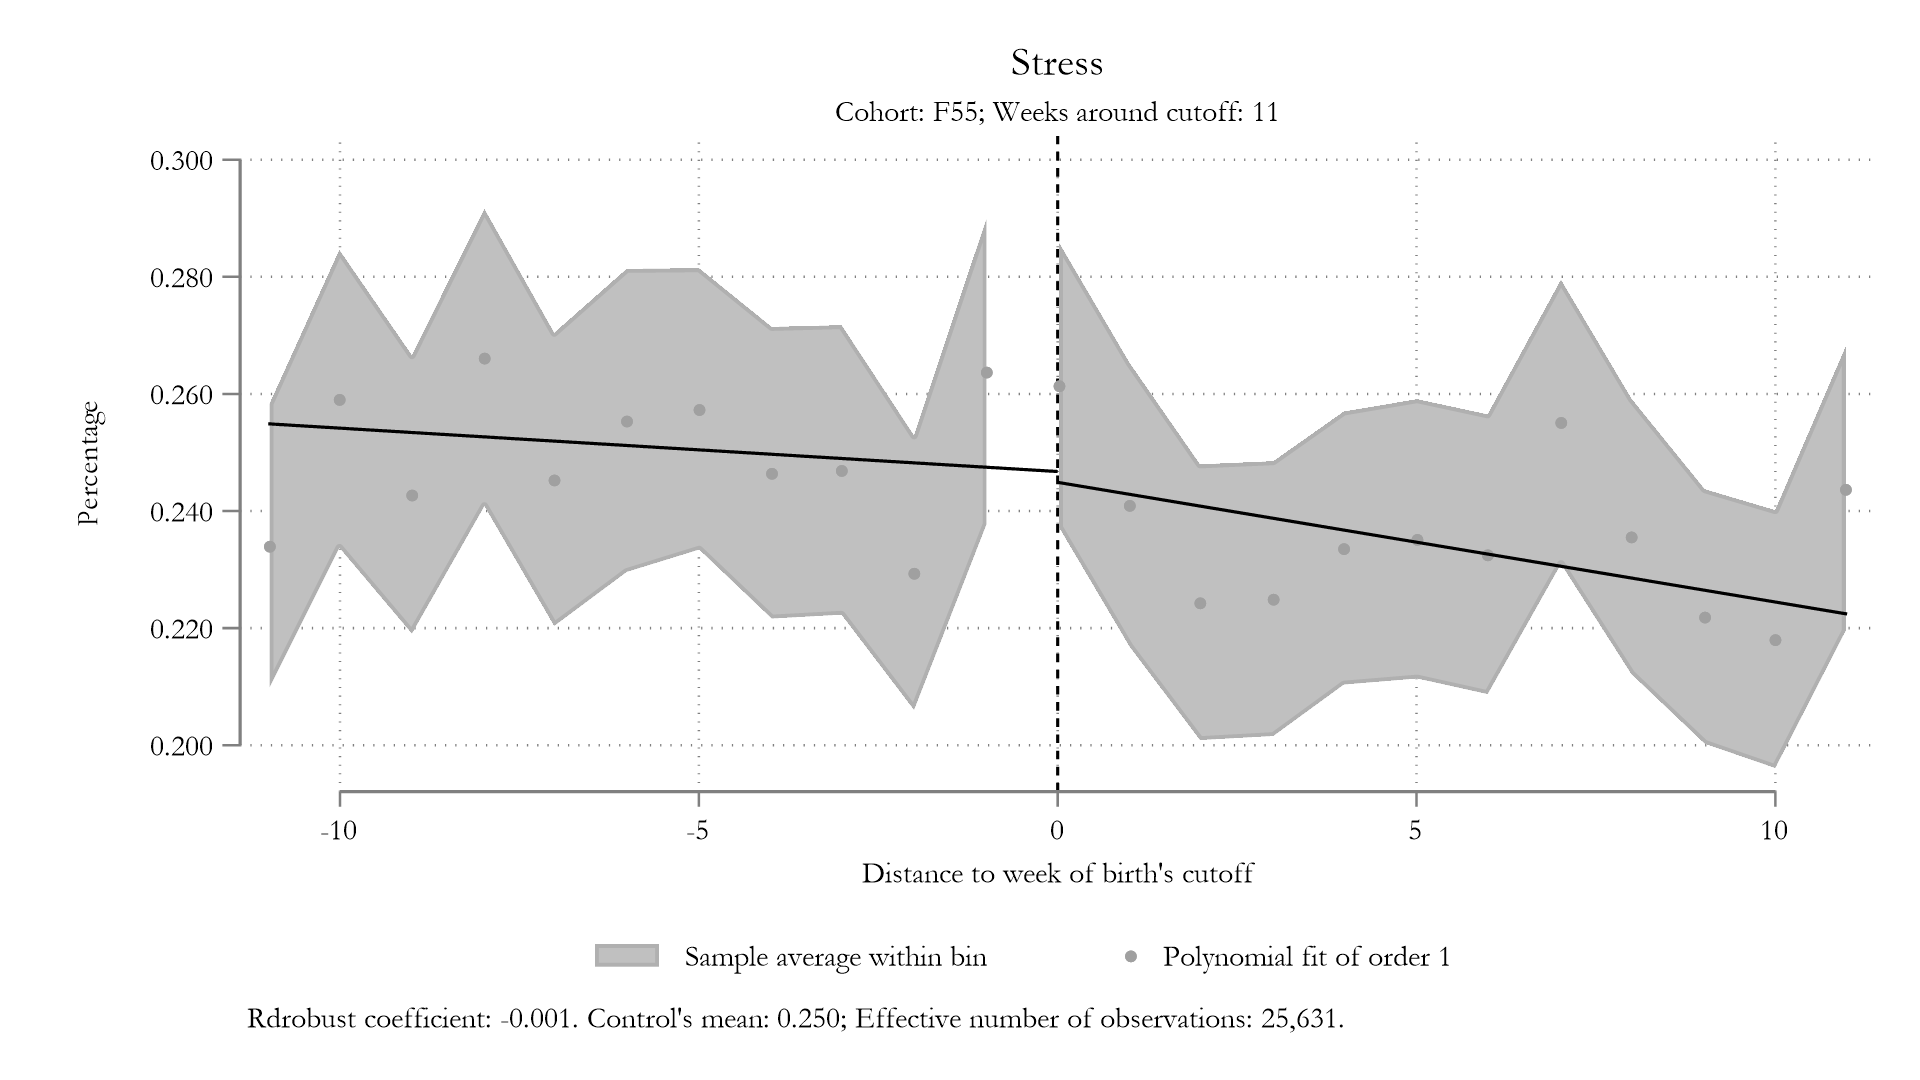
\includegraphics{Graphs/cumulative/estres_F55_11.png}
    }
    \vfill
    \centering
    \hyperlink{f55_stress}{\beamergotobutton{Back}}
\end{frame}

\begin{frame}[label=m50_stress_cum]{Health results}
    \centering
    \resizebox{0.8\textwidth}{!}{
      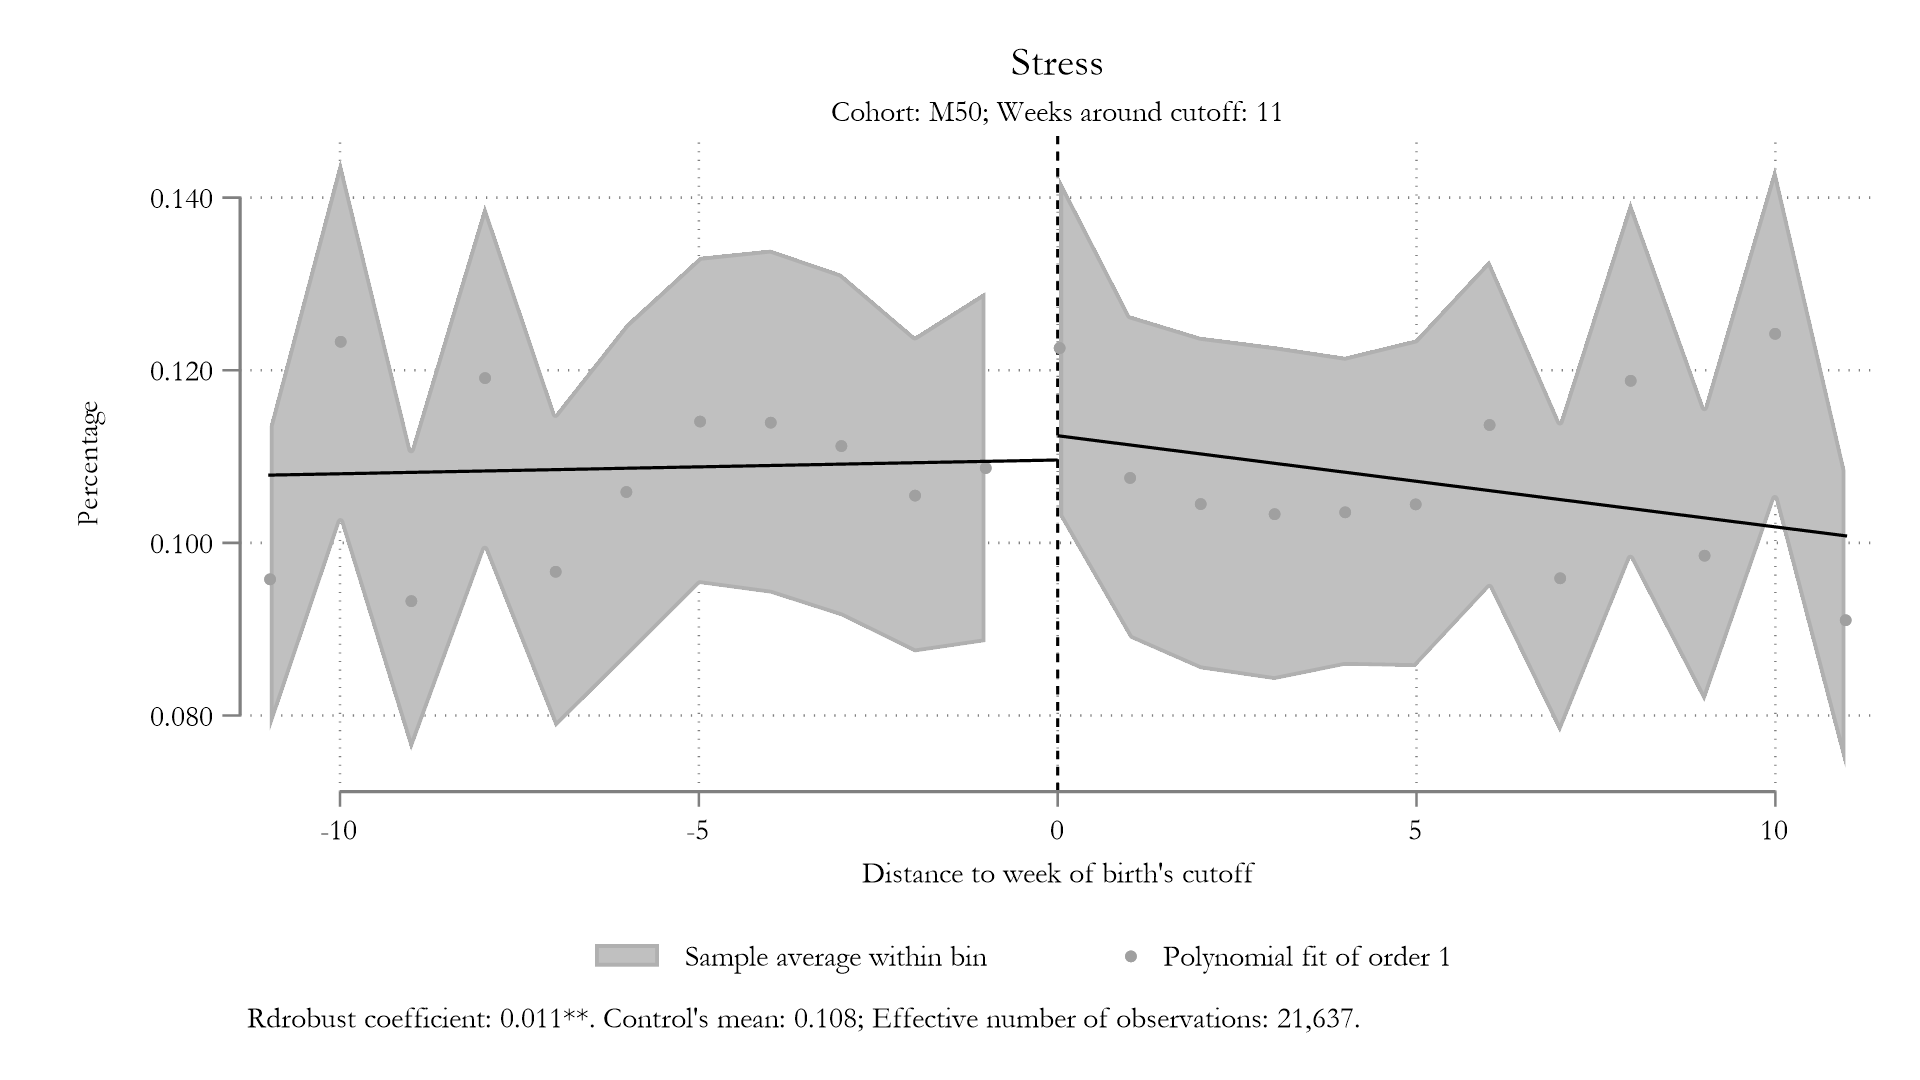
\includegraphics{Graphs/cumulative/estres_M50_11.png}
    }
    \vfill
    \centering
    \hyperlink{m50_stress}{\beamergotobutton{Back}}
\end{frame}


%% Mental diagnosis
\begin{frame}[label=f55_mental_cum]{Health results}
    \centering
    \resizebox{0.8\textwidth}{!}{
      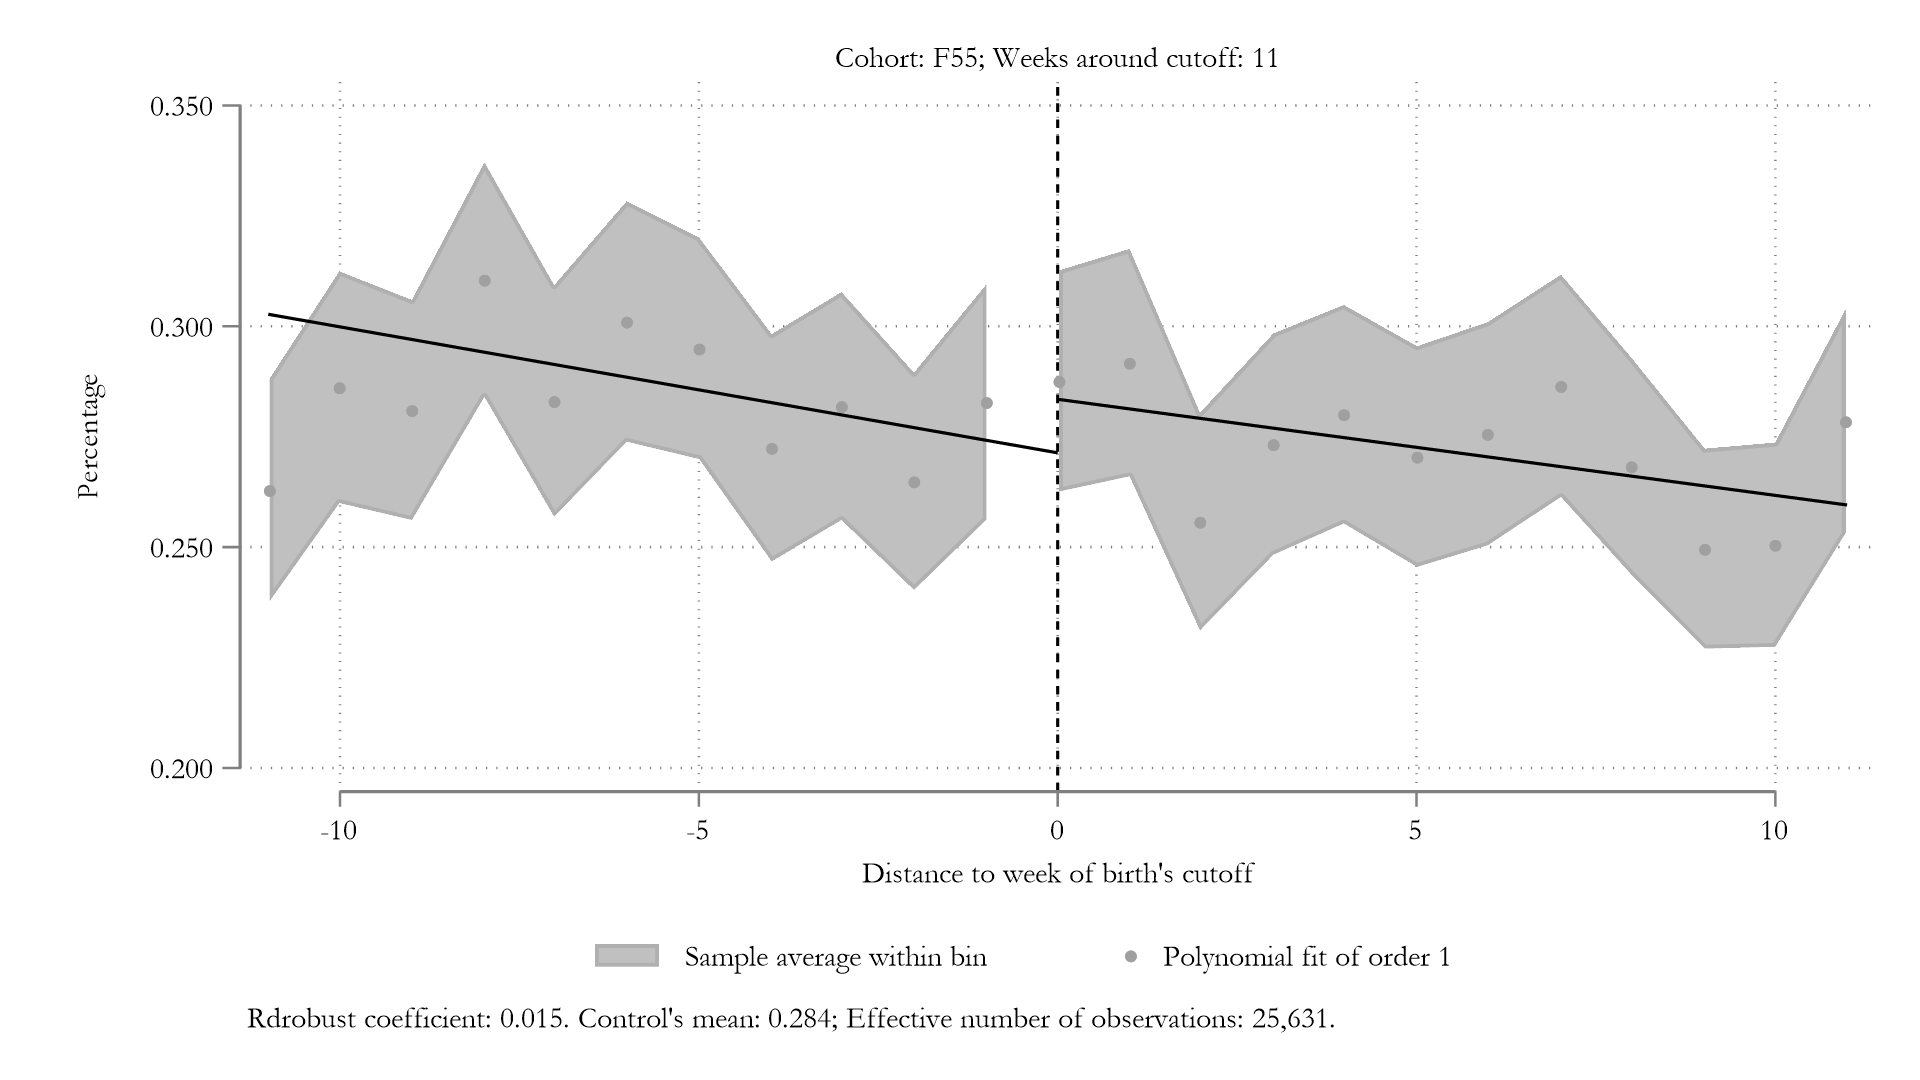
\includegraphics{Graphs/cumulative/diag_mental_F55_11.png}
    }
    \vfill
    \centering
    \hyperlink{f55_mental}{\beamergotobutton{Back}}
\end{frame}

\begin{frame}[label=m50_mental_cum]{Health results}
    \centering
    \resizebox{0.8\textwidth}{!}{
      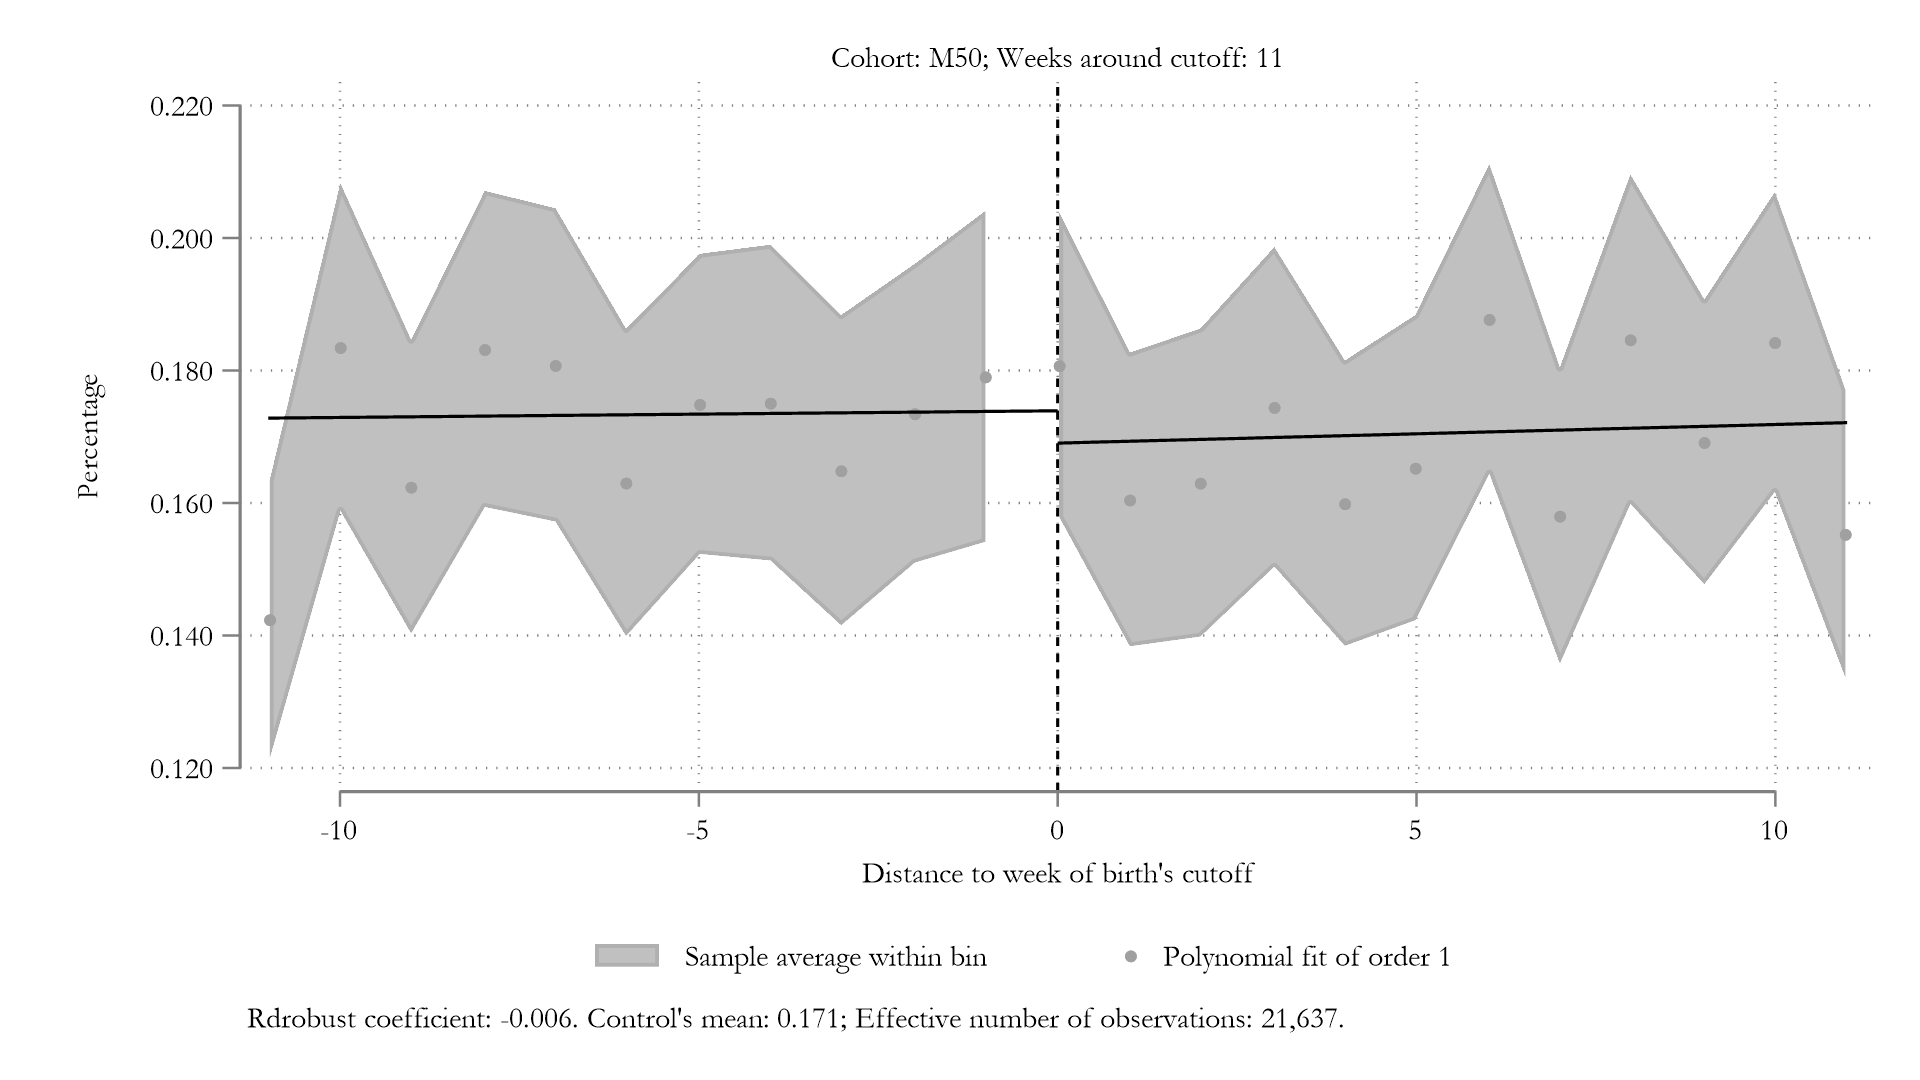
\includegraphics{Graphs/cumulative/diag_mental_M50_11.png}
    }
    \vfill
    \centering
    \hyperlink{m50_mental}{\beamergotobutton{Back}}
\end{frame}


%% MWI
\begin{frame}[label=f55_mwi_cum]{Health results}
    \centering
    \resizebox{0.8\textwidth}{!}{
      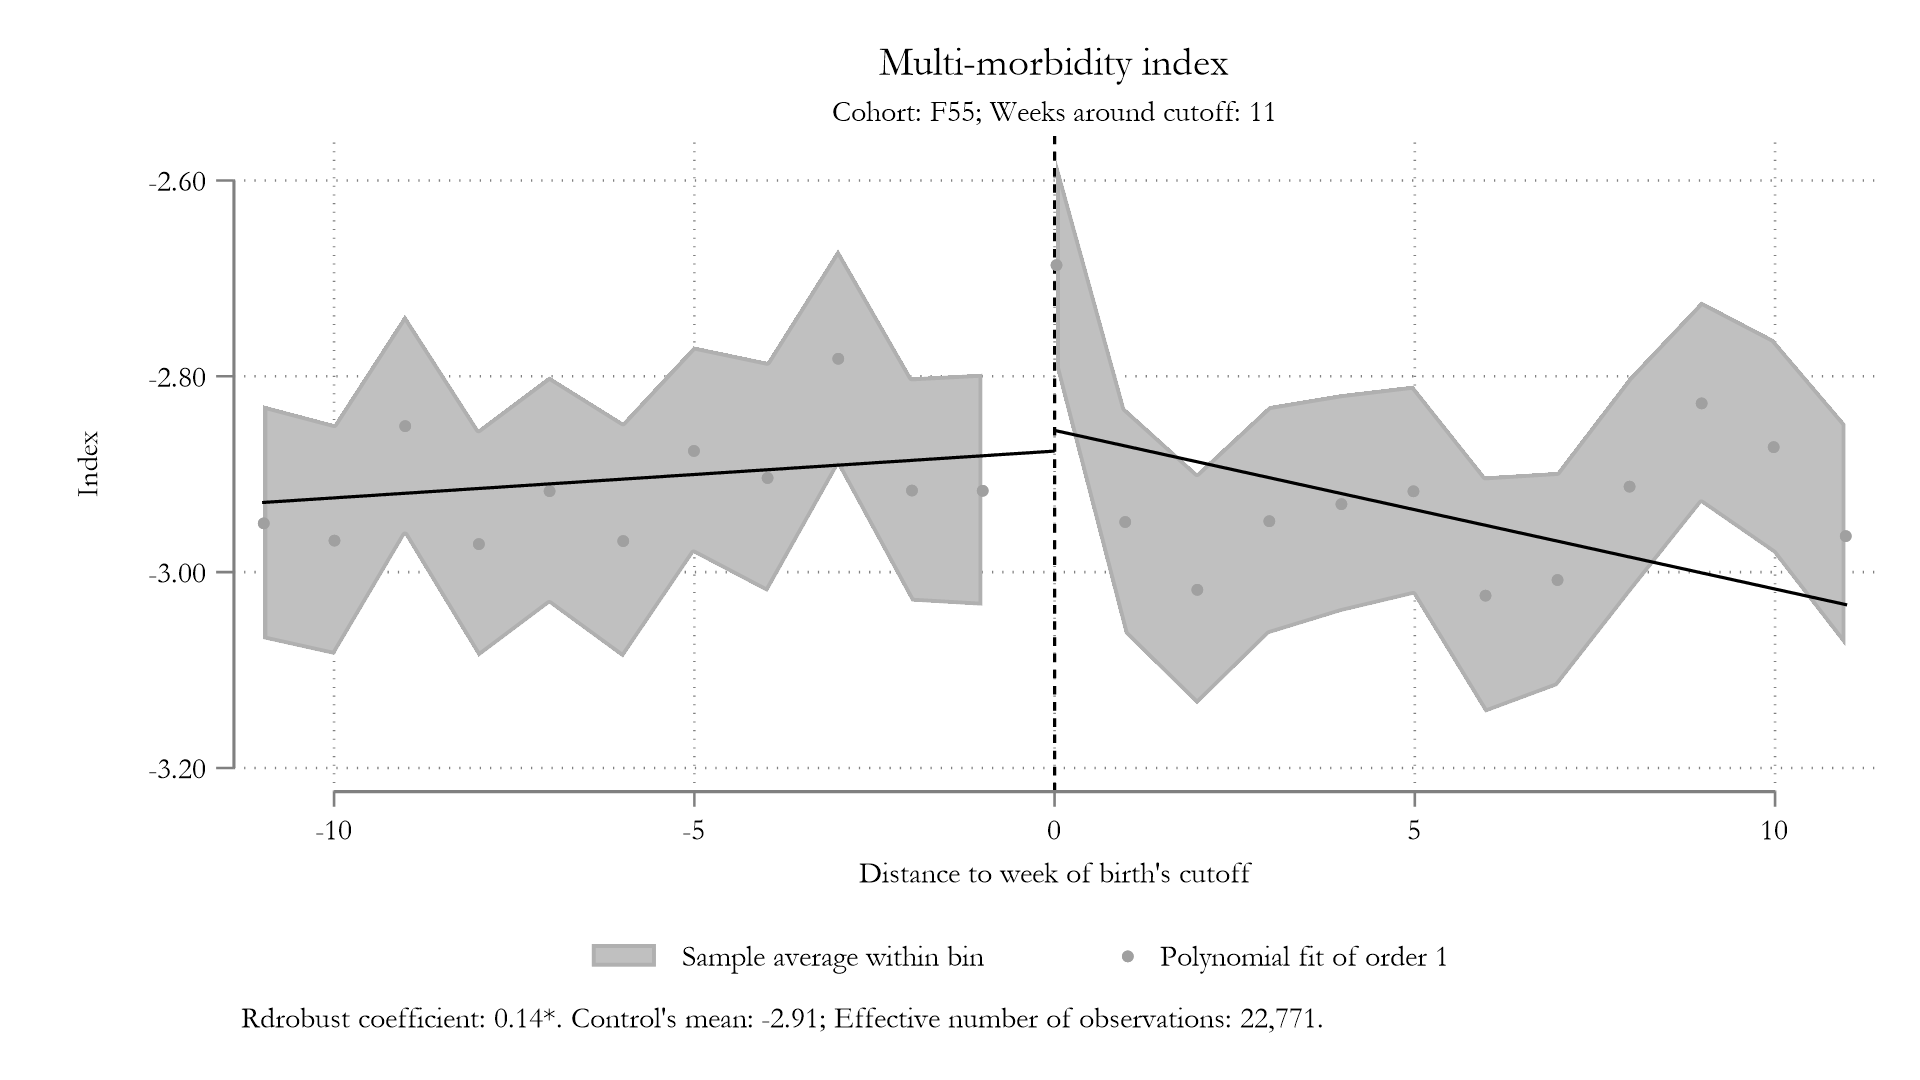
\includegraphics{Graphs/cumulative/pre_MWI_F55_11.png}
    }
    \vfill
    \centering
    \hyperlink{f55_mwi}{\beamergotobutton{Back}}
\end{frame}

\begin{frame}[label=m50_mwi_cum]{Health results}
    \centering
    \resizebox{0.8\textwidth}{!}{
      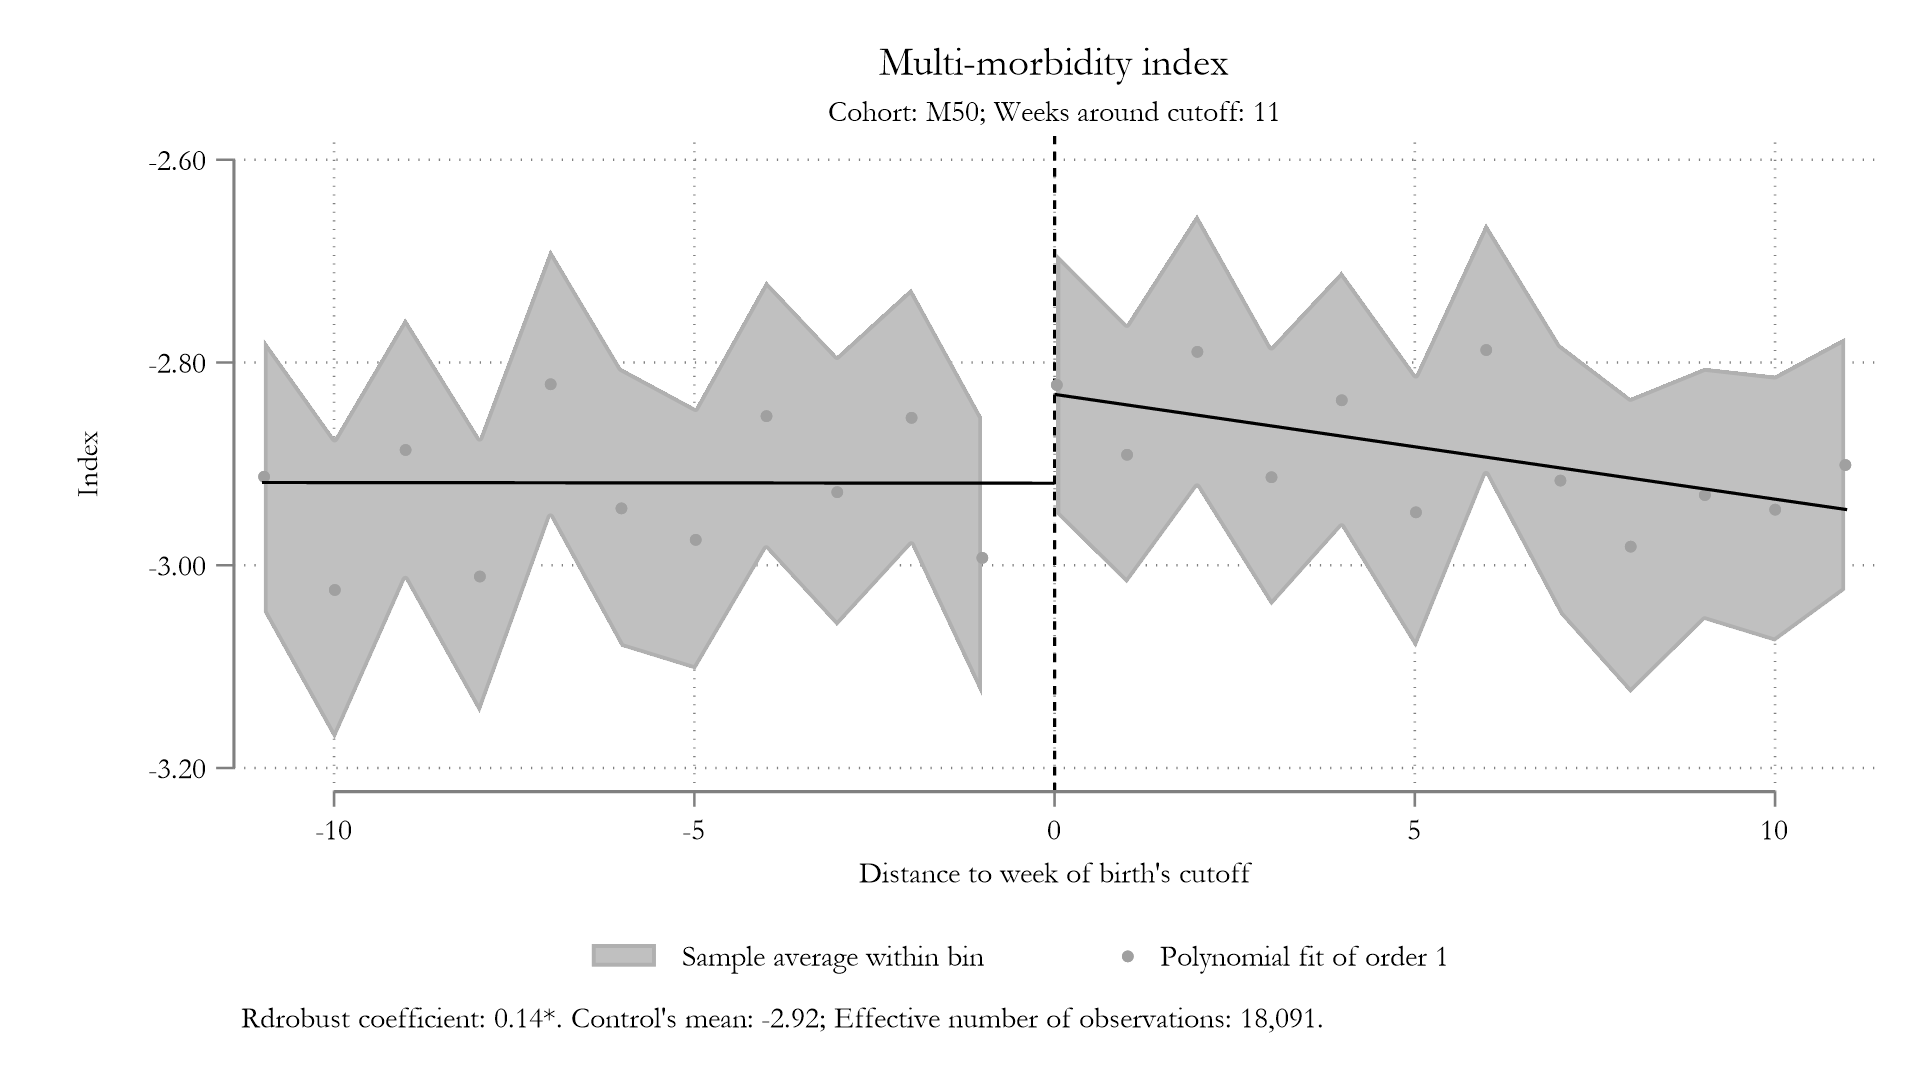
\includegraphics{Graphs/cumulative/pre_MWI_M50_11.png}
    }
    \vfill
    \centering
    \hyperlink{m50_mwi}{\beamergotobutton{Back}}
\end{frame}

\end{document}


